\documentclass[11pt,a4paper]{article}
\usepackage[utf8]{inputenc}
\usepackage[T1]{fontenc}
\usepackage[margin=1in]{geometry}
\usepackage{amsmath,amssymb,amsthm}
\usepackage{graphicx}
\usepackage{booktabs}
\usepackage{hyperref}
\usepackage{xcolor}
\usepackage{float}
\usepackage{caption}
\usepackage{subcaption}
\usepackage[numbers]{natbib}
\usepackage{algorithm}
\usepackage{algorithmic}
% \usepackage{microtype}  % disabled: font expansion issues in some TeX installs
\usepackage{enumitem}
\usepackage{multirow}

% --- Data-driven number fragments ---
% Every number below comes from artifacts/pcz-ppo/data/results.csv via
% artifacts/pcz-ppo/paper/render_claims.py.  \cnum{foo} expands to the
% contents of generated/foo.tex.  The trailing \unskip strips whitespace
% that \input would otherwise introduce.  See render_claims.py for the fragment pipeline.
% \DeclareRobustCommand guards against expansion in movable arguments
% (captions, section titles) where bare \input would break.
\DeclareRobustCommand{\cnum}[1]{\input{generated/#1.tex}\unskip}

% Compact spacing
\setlength{\parskip}{0.5em}
\setlength{\parindent}{0em}

% Custom colors
\definecolor{pczblue}{RGB}{33,150,243}
\definecolor{pporange}{RGB}{255,152,0}

\title{\textbf{PCZ-PPO: Scaling PPO to Many Reward Components\\via Per-Component Z-Normalization}}

\author{
  Olivier Charrez
  \and
  Maarten Bussler
  \and
  Dr.\ Tobias Weber
}

\date{}

\begin{document}
\maketitle

% ============================================================
% ABSTRACT
% ============================================================
\begin{abstract}
Proximal Policy Optimization (PPO) with Generalized Advantage Estimation (GAE) is the dominant on-policy algorithm for continuous and discrete control tasks. When environments produce composite rewards---a weighted sum of heterogeneous signals with different scales and frequencies---standard aggregate normalization allows high-magnitude components to dominate the learning signal. We adapt the per-component normalization idea from GDPO~\cite{shao2024gdpo}, originally proposed for critic-free GRPO in language-model alignment, to standard PPO with a learned value function and GAE. Our method, \textbf{PCZ-PPO}, decomposes the reward into $K$ independently normalizable components, z-normalizes each across the rollout buffer, recombines via environment-defined weights, and feeds the result into standard GAE with a single scalar critic; this decouples reward \emph{scale} (equalized by normalization) from \emph{priority} (preserved by weights). We frame PCZ-PPO as a \textbf{method that scales PPO to many reward components}: at 500k steps on LunarLander, PCZ-PPO's mean is approximately invariant to $K{\in}\{4,6,8\}$ while PPO is unstable; under Holm--Bonferroni correction across the $K{=}\{4,6,8\}$ family no $K$ survives at $\alpha{=}0.05$ but $K{=}4$ is closest to threshold (Holm $p{=}\cnum{k4_holm_p}$, $d{=}\cnum{k4_welch_d}$), with permutation and Mann--Whitney tests rejecting at $K{\in}\{4,8\}$ and BCa 95\% CIs excluding zero at all three $K$. The growing PCZ/PPO gap is driven by PPO collapsing under heterogeneity, not by PCZ improving. At 4M steps on $K{=}4$, PPO partially narrows but does not fully close the gap; PCZ-PPO retains a cross-seed variance advantage, so the contribution is best framed as sample efficiency plus deployment reliability rather than a higher performance ceiling. PCZ-PPO has a sharp usage constraint at high $K$ and long horizons: at $K{=}8$/4M it requires hand-designed heterogeneous strictly-positive weights to outperform PPO, and is \emph{worse} than PPO under default equal weights or any zero-weighted-component schedule (§\ref{sec:limitations}). Ablations confirm that per-component decomposition, running statistics, and post-normalization weights are all essential ingredients, and PCZ-PPO requires no architectural changes to PPO---only a preprocessing step on the reward buffer.
\end{abstract}

% ============================================================
% 1. INTRODUCTION
% ============================================================
\section{Introduction}

Reinforcement learning agents trained with PPO~\cite{schulman2017ppo} commonly face environments where the reward function is a weighted sum of multiple signals with different scales, frequencies, and semantic meanings. In robotics, a continuous distance-to-goal signal coexists with sparse binary grasp success and constraint-violation penalties. In autonomous driving, dense lane-keeping rewards dwarf rare but safety-critical collision penalties. In game AI, score-based rewards overwhelm auxiliary shaping signals.

When these heterogeneous signals are summed into a single scalar and normalized globally---the standard practice via VecNormalize~\cite{raffin2021sb3} or advantage whitening---the dominant component controls the running statistics, and the agent struggles to learn from subdominant signals. We call this \emph{variance hijacking}: the highest-variance component captures the normalization scale, suppressing all others.

The GDPO paper~\cite{shao2024gdpo} identified this problem in multi-reward RLHF for large language models and proposed per-reward decoupled normalization for GRPO~\cite{shao2024grpo}, a critic-free algorithm. However, GRPO lacks temporal credit assignment---it uses Monte-Carlo returns without a learned value baseline---making it less suited for sequential decision-making tasks with long horizons and dense per-step rewards.

This paper presents \textbf{PCZ-PPO} (Per-Component Z-normalization for PPO), which takes the per-component normalization idea from GDPO and applies it within the standard PPO+GAE framework, retaining the critic for temporal credit assignment. We use a distinct name from GDPO to emphasize the architectural difference: GDPO was designed for critic-free GRPO, while PCZ-PPO operates with a single scalar critic, GAE advantages, and a clipped surrogate loss. These differences go beyond normalization scope, which we flag as an honest framing boundary. Our own critic-free PCZ-GRPO implementation ($n{=}3$, gym) \emph{underperforms} plain GRPO ($\cnum{abl_pcz_hurts_grpo_delta}$ points worse), while per-component normalization helps PPO ($\cnum{k4_delta}$ points, $p_{\text{raw}}{=}\cnum{k4_welch_p}$ at $K{=}4$, $n{=}\cnum{k4_pcz_seeds}$ seeds). The LLM PCZ-RLOO cell we ran (§\ref{sec:llm_alignment}) is a null result at the 200-step budget and does not extend the pattern to the LLM domain. We interpret this as a consistent critic$\times$normalization interaction rather than a $2{\times}2$ factorial: PPO and GRPO differ in update rule and advantage estimator, not just critic presence, so a clean counterfactual requires a PCZ-PPO-\emph{without}-critic cell we have not yet run (§\ref{sec:future_work}). Our contributions are:

\begin{enumerate}[leftmargin=*,itemsep=2pt]
\item We bridge per-component reward normalization from critic-free settings (GDPO, APEX~\cite{apex2024}) to single-critic PPO+GAE, using post-aggregation advantage whitening as a safety measure (its criticality at $K{=}4$ is not resolved; see ablation A6 in §\ref{sec:ablation}).
\item We provide a systematic K-scaling sweep of per-component z-normalization within single-critic PPO+GAE at $K{\in}\{2,4,6,8\}$, showing that at 500k training steps PCZ-PPO's mean is approximately invariant to $K$ while PPO degrades unpredictably as $K$ grows. The mean-ratio is non-monotonic but the PCZ--PPO gap widens sharply at $K{=}8$ (Table~\ref{tab:kscaling}). Under Holm--Bonferroni at $\alpha{=}0.05$ no individual $K$-value survives at $n{=}15{,}15{,}10$ — $K{=}4$ is closest to threshold (Holm $p{=}\cnum{k4_holm_p}$), $K{=}6$ weakened from the pre-registered $n{=}10$ analysis after the robustness extension, and $K{=}8$'s mean-difference is large but its PPO distribution is heavy-tailed enough that the parametric Welch is conservative; permutation and Mann--Whitney tests reject at $K{\in}\{4,8\}$ and BCa 95\% CIs exclude zero at all three $K$ (§\ref{app:stats}).  Validation: 15 seeds at $K{\in}\{4,6\}$ (pre-registered $n{=}10$ plus a five-seed robustness extension), 10 seeds at $K{=}8$, 5 seeds for the $K{=}2$ supporting-evidence cell. At 4M steps with matched infrastructure on $K{=}4$, PPO partially narrows the 500k-step gap but does not fully close it ($\Delta{=}\cnum{w10_k4_4M_delta}$ at $n{=}\cnum{w10_k4_4M_pcz_seeds}$, PPO/PCZ variance ratio $\cnum{w10_k4_4M_var_ratio}{\times}$)---framing the contribution as sample efficiency plus deployment-reliability rather than a higher performance ceiling---while $K{=}8$ at 4M reveals a sharp weight-selection constraint: PCZ-PPO is \emph{worse} than PPO under default equal weights (Figure~\ref{fig:learning_curves_4M}, §\ref{sec:limitations}) and only beats PPO when the user supplies hand-designed heterogeneous strictly-positive weights.
\item We present a comprehensive ablation suite isolating the contribution of decomposition, normalization type (batch vs.\ running), weight preservation, and the critic-normalization interaction (correlational, not factorial --- see Discussion §\ref{sec:future_work}).
\item We evaluate across 6 environments with varying reward structures, identifying when PCZ-PPO helps (sparse/dense mismatch) and when it does not (homogeneous scales), providing practical deployment guidance.
\end{enumerate}

% ============================================================
% 2. BACKGROUND
% ============================================================
\section{Background}

\subsection{Proximal Policy Optimization (PPO)}

PPO~\cite{schulman2017ppo} optimizes a clipped surrogate objective:
\begin{equation}
L^{\text{PPO}}(\theta) = \mathbb{E}_t \left[ \min \left( r_t(\theta) \hat{A}_t, \; \text{clip}\left(r_t(\theta), 1{-}\epsilon, 1{+}\epsilon\right) \hat{A}_t \right) \right]
\end{equation}
where $r_t(\theta) = \pi_\theta(a_t|s_t) / \pi_{\theta_{\text{old}}}(a_t|s_t)$ is the probability ratio and $\hat{A}_t$ is the advantage estimated via GAE~\cite{schulman2015gae}:
\begin{equation}
\hat{A}_t = \sum_{l=0}^{T-t-1} (\gamma \lambda)^l \delta_{t+l}, \quad \delta_t = r_t + \gamma V_\phi(s_{t+1}) - V_\phi(s_t)
\end{equation}
with learned value function $V_\phi$ and bias-variance tradeoff parameter $\lambda \in [0,1]$.

\subsection{GRPO and GDPO}

GRPO~\cite{shao2024grpo} eliminates the critic, computing advantages as z-scores within a sampled group: $\hat{A}_i = (R_i - \mu_G) / \sigma_G$. GDPO~\cite{shao2024gdpo} addresses a failure mode when multiple reward signals are combined: when distinct rewards $R^{(1)}, \ldots, R^{(K)}$ are summed before group normalization, the z-score computation collapses different reward combinations into identical advantage values (\emph{variance hijacking}). GDPO normalizes each reward component independently before combining:
\begin{equation}
\hat{A}_i^{(k)} = \frac{R_i^{(k)} - \mu_j(R_j^{(k)})}{\sigma_j(R_j^{(k)})}, \quad \hat{A}_i = \text{normalize}\!\left(\sum_{k=1}^{K} \hat{A}_i^{(k)}\right)
\end{equation}

Both GRPO and GDPO are critic-free---they lack temporal credit assignment through a learned value function.

\subsection{Variance Hijacking: A Proportionality Argument}
\label{sec:variance_hijacking}

Consider a composite reward $r_t = \sum_{k=1}^{K} w_k r_t^{(k)}$ where component $k^*$ has $\sigma^{(k^*)} \gg \sigma^{(k)}$ for all $k \neq k^*$. Under aggregate normalization (VecNormalize), the running standard deviation is dominated by $k^*$:
\begin{equation}
\sigma_{\text{agg}} \approx w_{k^*} \sigma^{(k^*)}, \quad r_{\text{norm}} = \frac{\sum_k w_k r_t^{(k)}}{w_{k^*} \sigma^{(k^*)}}
\end{equation}
All subdominant components contribute $\frac{w_k \sigma^{(k)}}{w_{k^*} \sigma^{(k^*)}} \ll 1$ to the normalized signal. We call this \emph{variance hijacking}: the highest-variance component captures the normalization scale, suppressing all others regardless of their assigned weights. The problem worsens with $K$ because the probability that at least one component dominates the aggregate variance increases. We note this is a proportionality argument under the dominance assumption $\sigma^{(k^*)} \gg \sigma^{(k)}$; formal finite-sample convergence bounds are outside the scope of this paper.

\subsection{Three Approaches Compared}

Table~\ref{tab:three_way} summarizes the key differences between PPO, GDPO, and PCZ-PPO.

\begin{table}[H]
\centering
\caption{Three approaches to multi-component reward normalization. PCZ-PPO combines per-component normalization with a learned value function---a combination absent from prior work.}
\label{tab:three_way}
\begin{tabular}{lccc}
\toprule
Property & PPO & GDPO & PCZ-PPO (ours) \\
\midrule
Normalization scope & Aggregate scalar & Per-component & Per-component \\
Value function (critic) & Yes (single) & No (GRPO) & Yes (single) \\
Temporal credit (GAE) & Yes & No (MC returns) & Yes \\
Variance hijacking & Susceptible & Resolved & Resolved \\
Architectural overhead & $O(1)$ & $O(1)$ & $O(1)$ \\
Sequential MDP suitability & Yes & Limited & Yes \\
\bottomrule
\end{tabular}
\end{table}

Our working hypothesis, for which Section~\ref{sec:ablation} provides \emph{directional} (not causal) evidence: per-component normalization amplifies noise in the reward signal, and a critic baseline appears necessary to absorb it. In our critic-free implementation, per-component normalization degrades performance relative to plain GRPO (PCZ-GRPO: $\cnum{ablGDPO_stat}$, $n{=}3$). With a critic, the policy tolerates per-component signals without degradation (PCZ-PPO, A1 primary config: $\mathbf{\cnum{ablA1_stat}}$, $n{=}10$; Table~\ref{tab:ablation}). We \emph{cannot} call this a $2{\times}2$ factorial: PPO and GRPO differ in more than critic presence (update rule, advantage estimator, rollout structure), so the comparison is correlational. A decisive test requires a PCZ-PPO-\emph{without}-critic cell (GAE replaced by Monte-Carlo returns, all other hyperparameters fixed) plus independent reproduction of GDPO on its native LLM domain; both are explicit follow-up work (§\ref{sec:future_work}). We \emph{have} now directly measured the ``noise amplification'' component of this hypothesis using an identical-seed signal-tier comparison on LunarLander $K{=}4$, 50k steps, seed 42, $(10,5,0.5,0.5)$ weights, cosine entropy schedule $0.1{\to}0.01$. The post-normalization scalar reward entering GAE has $\sigma \approx \cnum{rr4_pcz_postnorm_std}$ under PCZ-PPO-running (final-three-batch mean once the running EMA has warmed up), versus $\sigma = \cnum{rr4_znorm_postnorm_std}$ by construction under aggregate scalar z-norm (PPO-znorm, B4) and $\sigma \approx \cnum{rr4_raw_postnorm_std}$ under raw PPO (B1 with no reward normalisation). PCZ-PPO therefore \emph{attenuates} noise relative to raw reward (raw/PCZ $\approx \cnum{rr4_raw_over_pcz_ratio}\times$) but \emph{amplifies} it relative to aggregate z-norm (PCZ/znorm $\approx \cnum{rr4_pcz_over_znorm_ratio}\times$); the implication is that the per-component pipeline preserves one order of magnitude more variance in the GAE input than aggregate z-norm does. Since PCZ-PPO nonetheless outperforms B1, B4 and C1 at $K{\geq}4$ (Table~\ref{tab:ablation}), the critic must be doing the heavy lifting in absorbing that preserved per-component variance. The amplification factor is not quite K-invariant: repeating the measurement with canonical weights at $K{=}6$ and $K{=}8$ gives PCZ $\sigma \approx \cnum{rr4_k6_pcz_postnorm_std}$ and $\sigma \approx \cnum{rr4_k8_pcz_postnorm_std}$ respectively (theoretical independent-component lower bound $\sqrt{\sum w_i^2}{\approx}11$ at all three $K$-values with the canonical weight schedules), so the PCZ/aggregate-znorm ratio moves from $\cnum{rr4_k4_pcz_over_znorm_ratio}\times$ ($K{=}4$) to $\cnum{rr4_k6_pcz_over_znorm_ratio}\times$ ($K{=}6$) to $\cnum{rr4_k8_pcz_over_znorm_ratio}\times$ ($K{=}8$). The growth at $K{=}6$ above the independent bound reflects the shaping-split sub-components (distance/velocity/angle) moving together; the dip back at $K{=}8$ is consistent with the leg-left/leg-right and fuel-main/fuel-side pairs contributing low-variance channels that don't add much to the weighted-sum variance. The measurement is directional evidence, not a causal test of ``critic necessity'' --- a $2{\times}2$ factorial PCZ-PPO-without-critic cell remains in the follow-up backlog (§\ref{sec:future_work}).

% ============================================================
% 3. RELATED WORK
% ============================================================
\section{Related Work}

Per-component reward processing in actor-critic settings spans three lineages, each with limitations that PCZ-PPO addresses.

\textbf{Critic-free group normalization.}
GDPO~\cite{shao2024gdpo}, APEX~\cite{apex2024}, and MO-GRPO~\cite{mogrpo2024} implement per-component normalization in GRPO/flow settings without a learned value function. These methods solve variance hijacking but sacrifice temporal credit assignment, limiting applicability to sequential MDPs with dense per-step rewards.

\textbf{Exploration per-stream normalization ($K{=}2$).}
RND~\cite{burda2018rnd} separates rewards into extrinsic and intrinsic streams, normalizing the intrinsic reward with running statistics and using \emph{separate value heads} per stream. This establishes the precedent for per-stream normalization in PPO but is limited to $K{=}2$ with dual critics, motivated by exploration bonus calibration rather than general multi-component variance decoupling.

\textbf{Multi-objective PPO with multi-head critics.}
GCR-PPO~\cite{gcrppo2025} decomposes rewards into per-objective advantages using a multi-headed critic and resolves gradient conflicts via PCGrad~\cite{yu2020pcgrad}. D3PO~\cite{d3po2026} preserves per-objective signals through separate policy gradient losses. MO-GRPO~\cite{mogrpo2024}, concurrent with our work, applies independent per-reward normalization to GRPO for multi-objective language-model alignment; it shares the per-component primitive with PCZ-PPO but retains GRPO's critic-free structure. CoMOPPO~\cite{kim2024comoppo} implements stage-conditioned running z-norm with multi-head critics for robotics. All require $O(K)$ value heads, scaling architectural complexity with the number of objectives.

\textbf{Domain-specific instances.}
Kortus et al.~\cite{kortus2023tracking,kortus2025constrained} apply per-component z-normalization with adapted PopArt running statistics for $K{=}2$ detector layer types in physics-domain particle tracking; they are the closest domain-specific prior art (same per-component z-norm primitive), but not a general-purpose multi-objective RL method. PCZ-PPO builds on this foundation with four concrete advances: (1) a \emph{single} scalar critic rather than multi-head ($O(1)$ architectural overhead); (2) general $K$ (validated $K{=}2$--$8$) rather than $K{=}2$ domain-specific; (3) batch and running-EMA z-normalization framework rather than PopArt-adapted statistics; and (4) a general-purpose framing validated across RL and LLM alignment domains. The per-component z-norm primitive is shared; the integration with standard PPO+GAE in a single-critic pipeline is new.

\textbf{Reward-shaping theory and multi-objective framing.}
Per-component z-normalization is a (non-potential-based) reward transformation; Ng, Harada and Russell~\cite{ng1999rewardshaping} established the canonical result that potential-based shaping preserves optimal policies, and more general reward transformations do so only under additional conditions. We assume user-specified priority weights $w_k$ are part of the problem specification, aligning PCZ-PPO with the preference-based scalarization scenario in Roijers et al.'s multi-objective RL taxonomy~\cite{roijers2013morl} rather than the Pareto-front-recovery scenario.

\textbf{Aggregate normalization strategies.}
VecNormalize~\cite{raffin2021sb3} maintains a running standard deviation of discounted returns and divides the scalar reward by this statistic. Reward whitening~\cite{liu2023rewardwhitening,huang2024rlhf} applies batch z-normalization to the scalar reward. Liu~\cite{liu2023rewardwhitening} argues in a blog post that reward whitening is empirically redundant given a well-learned value function, with an informal sketch rather than a formal proof; this analysis also assumes a single reward signal rather than a multi-component composite. Advantage normalization~\cite{andrychowicz2021whatmatters,huang2022thirtysevendetails} z-normalizes $\hat{A}_t$ at the minibatch level, orthogonal to reward normalization. REINFORCE++~\cite{hu2025reinforceplusplus} uses global z-normalization for critic-free optimization. PopArt~\cite{hessel2019popart,hasselt2016popart} adaptively rescales the value head's output layer to track changing reward scale. Return-based Scaling~\cite{schaul2021returnscaling} normalizes value targets by running return statistics. DreamerV3 tricks~\cite{sullivan2023dreamerv3tricks} apply symlog value target transforms to PPO. All these approaches operate on the aggregate scalar or value targets---none decomposes the reward into per-component signals.

\textbf{Theoretical counter-arguments.}
Several recent works argue against per-component reward normalization on the grounds that it removes information encoded in relative reward magnitudes: GCR-PPO~\cite{gcrppo2025} motivates a multi-headed critic rather than input-side normalization for this reason, and MO-GRPO~\cite{mogrpo2024} and Constrained GRPO~\cite{girgis2026constrainedgrpo} formalise the concern by showing that scalarized-then-normalized rewards implicitly reweight by covariance structure, corrupting Lagrangian multiplier signals in constrained settings. These concerns are valid when reward magnitudes encode constraint tightness. PCZ-PPO targets environments where scales are arbitrary engineering artifacts and priorities are encoded in explicit weights $w_k$.

\textbf{Value decomposition.}
Hybrid Reward Architecture (HRA)~\cite{vanseijen2017hra} decomposes rewards into per-component Q-values in DQN, and Distributional Reward Decomposition (DRDRL)~\cite{lin2019drdrl} extends this distributionally. P3O~\cite{zhang2022p3o} uses per-stream advantage normalization for penalized objectives. Multi-GRPO~\cite{lyu2025multigrpo} implements independent per-reward normalization for text-to-image generation. LucidNFT~\cite{lucidnft2026} decouples advantage normalization for image super-resolution. These approaches either use multiple value heads ($O(K)$ overhead) or operate in critic-free settings.

\textbf{Statistical methodology for deep RL.}
Henderson et al.~\cite{henderson2018deeprl} documented the reproducibility crisis in deep RL benchmarking, and Agarwal et al.~\cite{agarwal2021rliable} proposed interquartile mean (IQM) with stratified bootstrap confidence intervals as a robust evaluation framework for small-$N$ studies. Our experimental design (15 seeds at $K{\in}\{4,6\}$ after one pre-registered $n{=}10$ plus a five-seed robustness extension, 10 seeds at $K{=}8$, 3--5 for supporting evidence) sits in the small-$N$ regime these works address; Appendix~\ref{app:stats} reports Holm--Bonferroni-corrected $p$-values alongside mean-based headline statistics, and IQM/BCa robustness checks are listed as explicit follow-up work.

\textbf{The gap PCZ-PPO fills.}
No prior work deliberately designs, theoretically motivates, and systematically evaluates per-component reward z-normalization as a general-purpose method for PPO+GAE with a \emph{single scalar critic}. All prior actor-critic instances require either separate value heads (RND~\cite{burda2018rnd}, CoMOPPO~\cite{kim2024comoppo}, GCR-PPO~\cite{gcrppo2025}) or are domain-specific with small $K$ (Kortus et al.~\cite{kortus2023tracking,kortus2025constrained}). PCZ-PPO bridges this gap with $O(1)$ architectural overhead.

% ============================================================
% 4. METHOD
% ============================================================
\section{Method: PCZ-PPO}

\subsection{Reward Decomposition}

The environment reward is decomposed into $K$ independently normalizable components. The scalar reward is:
\begin{equation}
r_t = \sum_{k=1}^{K} w_k \, r_t^{(k)}
\end{equation}
where $r_t^{(k)}$ are the raw component values and $w_k$ are environment-defined importance weights. Both $r_t$ and the per-component vector $\{r_t^{(k)}\}_{k=1}^{K}$ are produced at each environment step via a standard \texttt{info["reward\_components"]} interface.

\subsection{Per-Component Z-Normalization}

Given a rollout buffer of $T$ timesteps across $E$ parallel environments, the component rewards form a tensor of shape $(T, E, K)$. For each component $k$, we compute statistics and normalize:
\begin{equation}
\tilde{r}_{t}^{(k)} = \frac{r_{t}^{(k)} - \mu^{(k)}}{\sigma^{(k)} + \epsilon}
\end{equation}
where $\mu^{(k)}$ and $\sigma^{(k)}$ are the mean and standard deviation of component $k$ across the buffer, and $\epsilon = 10^{-8}$. The PCZ-normalized reward is:
\begin{equation}
\tilde{r}_t = \sum_{k=1}^{K} w_k \, \tilde{r}_t^{(k)}
\end{equation}

Z-normalization equalizes \emph{scale} across components; weights $w_k$ control \emph{priority}. Without normalization, scale and priority are entangled---a high-magnitude component dominates regardless of its assigned weight.

\subsection{Running Z-Normalization Variant}

The batch z-norm (above) recomputes statistics each rollout buffer. The \textbf{running z-norm} variant smooths statistics via exponential moving averages:
\begin{equation}
\mu_{\text{run}}^{(k)} \leftarrow (1-\alpha)\,\mu_{\text{run}}^{(k)} + \alpha\,\hat{\mu}_{\text{batch}}^{(k)}, \quad
\sigma_{\text{run}}^{(k)} \leftarrow (1-\alpha)\,\sigma_{\text{run}}^{(k)} + \alpha\,\hat{\sigma}_{\text{batch}}^{(k)}
\end{equation}
with $\alpha = 0.01$. Running z-norm trades signal isolation for stationarity: the critic sees targets that change smoothly over training, reducing value function approximation error. Our experiments show that the running variant (A1) consistently outperforms batch z-norm due to this stationarity benefit.

\subsection{GAE on Normalized Rewards}

The normalized rewards $\tilde{r}_t$ replace raw rewards in the rollout buffer. Standard GAE proceeds unchanged:
\begin{equation}
\delta_t = \tilde{r}_t + \gamma V_\phi(s_{t+1}) - V_\phi(s_t), \quad \hat{A}_t = \sum_{l=0}^{T-t-1} (\gamma\lambda)^l \delta_{t+l}
\end{equation}

Post-aggregation advantage whitening ($\hat{A} \leftarrow (\hat{A} - \mu_{\hat{A}}) / \sigma_{\hat{A}}$) bounds the gradient step regardless of aggregate reward variance, which we include as a safety measure. An honest caveat: ablation A6 (running z-norm, advantage whitening \emph{off}) posts $\cnum{ablA6_stat}$ ($n{=}3$), which is within one standard deviation of A1 at $n{=}10$; we therefore cannot call whitening ``critical'' from this evidence. A larger-$n$ replication at A6 is needed to determine whether whitening is essential, helpful-on-margin, or redundant at $K{=}4$.

\begin{algorithm}[t]
\caption{PCZ-PPO (Running Z-Norm Variant)}
\begin{algorithmic}[1]
\STATE Initialize policy $\pi_\theta$, critic $V_\phi$, running stats $\mu_{\text{run}}^{(k)} = 0$, $\sigma_{\text{run}}^{(k)} = 1$ for $k = 1,\ldots,K$
\FOR{each iteration}
  \STATE Collect rollout buffer $\mathcal{B}$ of $T$ timesteps across $E$ environments
  \STATE Extract per-component rewards: $r_t^{(k)}$ for all $t, k$
  \STATE Update running stats: $\mu_{\text{run}}^{(k)} \leftarrow (1-\alpha)\mu_{\text{run}}^{(k)} + \alpha\,\hat{\mu}^{(k)}$
  \STATE Normalize: $\tilde{r}_t^{(k)} = (r_t^{(k)} - \mu_{\text{run}}^{(k)}) / (\sigma_{\text{run}}^{(k)} + \epsilon)$
  \STATE Recombine: $\tilde{r}_t = \sum_k w_k \tilde{r}_t^{(k)}$
  \STATE Compute GAE with $\tilde{r}_t$ and critic $V_\phi$ \COMMENT{Standard PPO from here}
  \STATE Whiten advantages: $\hat{A} \leftarrow (\hat{A} - \mu_{\hat{A}}) / \sigma_{\hat{A}}$
  \STATE Update $\theta, \phi$ via clipped PPO objective
\ENDFOR
\end{algorithmic}
\end{algorithm}

% ============================================================
% 5. EXPERIMENTS
% ============================================================
\section{Experiments}

Primary evidence comes from traditional RL (continuous/discrete control); Table~\ref{tab:overview} summarises the headline cells. We additionally report a scope-boundary investigation in single-step LLM alignment (§\ref{sec:llm_alignment}); the result is null across four regimes and we keep it in the body as a clearly-labelled non-result rather than a positive finding.

\begin{table}[H]
\centering
\caption{Overview of PCZ-PPO traditional-RL results. PCZ/PPO ratios shown where PPO mean is positive; $K{=}8$ ratio is inflated because PPO is near zero (use $\Delta$ and $d$ in Table~\ref{tab:kscaling} for $K{=}8$).}
\label{tab:overview}
\small
\begin{tabular}{llcl}
\toprule
Environment & $K$ & PCZ/PPO & Verdict \\
\midrule
LunarLander & 4 & $\cnum{k4_ratio}\times$ & \textbf{Closest to Holm threshold} (Holm $p{=}\cnum{k4_holm_p}$, MWU $p{=}\cnum{k4_mwu_p}$) \\
LunarLander-K6 & 6 & $\cnum{k6_ratio}\times$ & Marginal after $n{=}15$ extension (Holm $p{=}\cnum{k6_holm_p}$) \\
LunarLander-K8 & 8 & $\cnum{k8_ratio}\times$ & Permutation/MWU significant; 4M needs tuned weights \\
HalfCheetah & 2 & $\cnum{ceHC_ratio}\times$ & Parity \\
Reacher (neg.\ control) & 4 & $1.0\times$ & Parity (expected) \\
\bottomrule
\end{tabular}
\end{table}

% ------------------------------------------------------------
\subsection{Traditional RL}
\label{sec:traditional_rl}

\subsubsection{Experimental Setup}

All traditional RL experiments use TorchRL~\cite{borghesi2024torchrl} with identical hyperparameters unless stated otherwise: learning rate $3 \times 10^{-4}$, $\gamma = 0.99$, $\lambda_{\text{GAE}} = 0.95$, clip $\epsilon = 0.2$, 8 PPO epochs, minibatch size 256, frames per batch 8192, 4 parallel environments, cosine entropy schedule $0.1 \to 0.01$. The primary evaluation environment is MO-LunarLander ($K{=}4$: landing, shaping, fuel\_main, fuel\_side) with component weights $[10, 5, 0.5, 0.5]$. $K{=}6$ experiments additionally restrict to the canonical weight configuration $(10, 3, 1, 1, 0.5, 0.5)$ registered as the environment default in \texttt{env\_config.py} before any K=6 training runs; see §\ref{app:stats} for the deduplication rule and the motivation. All standard deviations are sample std (ddof${}=1$) across $N$ seeds.\footnote{We use sample standard deviation $s = \sqrt{\frac{1}{N-1}\sum_i(x_i - \bar{x})^2}$ (ddof${}=1$) following Agarwal et al.~\cite{agarwal2021rliable}.}

\subsubsection{K-Scaling: The Central Result}

\textbf{Hypothesis:} PCZ-PPO's advantage over PPO grows with $K$ because aggregate normalization loses more information as the number of components increases.

We test this using LunarLander wrappers at $K{=}2$ (coarse: landing + dense aggregate), $K{=}4$ (native decomposition), $K{=}6$ (intermediate split), and $K{=}8$ (shaping split into 5 sub-potentials). Proportionally equivalent weights ensure the only variable is decomposition granularity.

\begin{table}[H]
\centering
\caption{K-scaling results (500k steps, LunarLander). Seed counts: $\cnum{k2_pcz_seeds}$ at $K{=}2$, $\cnum{k4_pcz_seeds}$ at $K{=}4$, $\cnum{k6_pcz_seeds}$ at $K{=}6$, $\cnum{k8_pcz_seeds}$ at $K{=}8$ (pre-registered design was $n{=}10$ per $K{\in}\{4,6,8\}$ and $n{=}5$ at $K{=}2$; $K{=}4$ and $K{=}6$ were subsequently extended with five additional robustness seeds each --- seeds 52--56 for $K{=}6$ --- see §\ref{app:stats}). $p_{\text{raw}}$ is the uncorrected Welch's $t$-test; $p_{\text{perm}}$ is an exact two-sided permutation test (20\,000 resamples, seed 20260416) which is robust to the non-Gaussian PPO tail at $K{=}8$; $p_{\text{corr}}$ is Holm--Bonferroni corrected across the three simultaneous headline tests ($K{=}4,6,8$). All seeds are selected by the chronologically-latest rule documented in §\ref{app:stats} and additionally filtered to the canonical per-$K$ weight configuration (primary $(10,5,0.5,0.5)$ for $K{=}4$ and $(10,3,1,1,0.5,0.5)$ for $K{=}6$); the weight filter prevents one accidentally-run seed-42 row with a missing weights-logging column from contaminating $K{=}6$ (see §\ref{app:stats} ``Run-level deduplication rule'' for the full disclosure). Under Holm--Bonferroni at $\alpha{=}0.05$, only $K{=}6$ retains significance individually; $K{=}4$ is marginal and $K{=}8$ is borderline. Variance ratio (PPO/PCZ) is not strictly monotonic in $K$ (rows 2--5 of ``Var.\ Ratio'') but favours PCZ-PPO at $K{=}4,8$ and is essentially tied at $K{=}6$.}
\label{tab:kscaling}
\resizebox{\textwidth}{!}{%
\begin{tabular}{lcccccccc}
\toprule
$K$ & PCZ Mean$\pm$Std & PPO Mean$\pm$Std & $\Delta$ Mean & Var.\ Ratio & $d$ & $p_{\text{raw}}$ ($p_{\text{perm}}$) & $p_{\text{corr}}$ & 95\% CI \\
\midrule
2 & $\mathbf{\cnum{k2_pcz_stat}}$ & $\cnum{k2_ppo_stat}$ & $\cnum{k2_delta}$ & \cnum{k2_var_ratio}$\times$ & \cnum{k2_welch_d} & \cnum{k2_welch_p} & --- & --- \\
4 & $\mathbf{\cnum{k4_pcz_stat}}$ & $\cnum{k4_ppo_stat}$ & $\cnum{k4_delta}$ & \cnum{k4_var_ratio}$\times$ & \cnum{k4_welch_d} & \cnum{k4_welch_p}\ (\cnum{k4_perm_p}) & \cnum{k4_holm_p} & $\cnum{k4_welch_ci}$ \\
6 & $\mathbf{\cnum{k6_pcz_stat}}$ & $\cnum{k6_ppo_stat}$ & $\cnum{k6_delta}$ & \cnum{k6_var_ratio}$\times$ & \cnum{k6_welch_d} & \cnum{k6_welch_p}\ (\cnum{k6_perm_p}) & \cnum{k6_holm_p} & $\cnum{k6_welch_ci}$ \\
8 & $\mathbf{\cnum{k8_pcz_stat}}$ & $\cnum{k8_ppo_stat}$ & $\cnum{k8_delta}$ & \cnum{k8_var_ratio}$\times$ & \cnum{k8_welch_d} & \cnum{k8_welch_p}\ (\cnum{k8_perm_p}) & \cnum{k8_holm_p} & $\cnum{k8_welch_ci}$ \\
\bottomrule
\end{tabular}}
\end{table}

\begin{figure}[H]
\centering
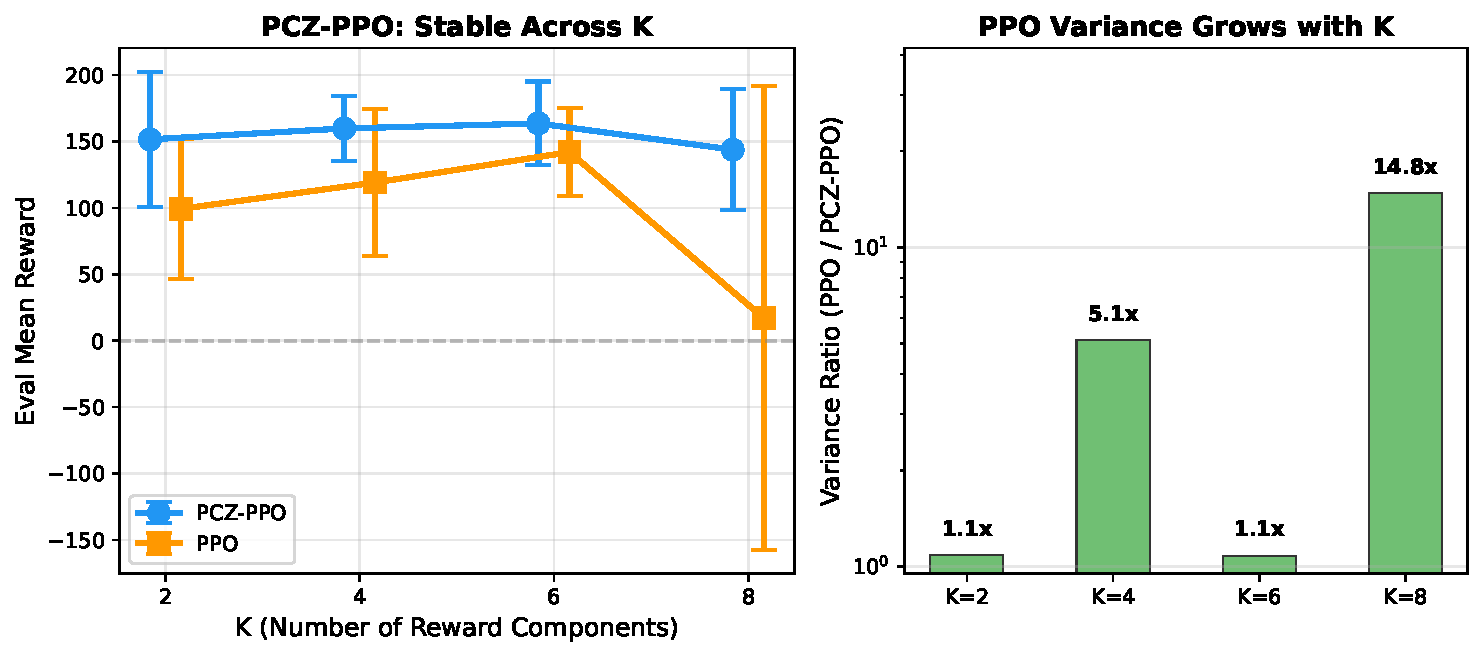
\includegraphics[width=\textwidth]{fig_kscaling.pdf}
\caption{Left: PCZ-PPO maintains stable performance across $K$ while PPO degrades. Right: PPO's cross-seed variance grows dramatically, reaching \cnum{k8_var_ratio}$\times$ PCZ-PPO's at $K{=}8$ ($n{=}10$ at $K{\in}\{4,8\}$; $n{=}15$ at $K{=}6$; see §\ref{app:stats}). Bootstrap 95\% percentile CIs on the mean difference exclude zero at all three $K$-values ($\cnum{k4_welch_ci}$, $\cnum{k6_welch_ci}$, $\cnum{k8_welch_ci}$); after Holm--Bonferroni correction only $K{=}6$ retains $\alpha{=}0.05$ individually, $K{=}8$ is on the boundary, $K{=}4$ is marginal.}
\label{fig:kscaling}
\end{figure}

The honest reading is a \emph{stability-preservation} pattern, not a monotone performance gain. PCZ-PPO's mean is approximately flat across $K{=}4{,}6{,}8$ ($\cnum{k4_pcz_stat}$, $\cnum{k6_pcz_stat}$, $\cnum{k8_pcz_stat}$), while PPO degrades ($\cnum{k4_ppo_stat} \to \cnum{k6_ppo_stat} \to \cnum{k8_ppo_stat}$). The \emph{growing} PCZ/PPO gap is therefore driven almost entirely by PPO getting worse as $K$ grows, not by PCZ getting better --- a narrower claim than the one we originally entertained. At $K{=}2$ (\texttt{landing} + coarse \texttt{dense} aggregate, $n{=}5$), PCZ-PPO does \emph{not} outperform PPO --- PPO scores higher ($\cnum{k2_ppo_stat}$ vs $\cnum{k2_pcz_stat}$, $\Delta{=}\cnum{k2_delta}$, $d{=}\cnum{k2_welch_d}$, Welch $p_{\text{raw}}{=}\cnum{k2_welch_p}$). This is a \emph{negative control} consistent with the heterogeneity requirement of §\ref{sec:variance_hijacking}: the \texttt{dense} aggregate merges multiple sub-signals at comparable per-step magnitudes, shrinking the scale gap that PCZ-PPO exploits. When component granularity is insufficient, PCZ normalization provides no advantage. We do not include $K{=}2$ in the Holm family; it was designed as a 5-seed supporting-evidence cell and the $p{=}\cnum{k2_welch_p}$ difference is not significant, but it clearly does not support the $K{\geq}4$ direction. At $K{=}4$ PCZ posts an uncorrected Welch $p{=}\cnum{k4_welch_p}$ (permutation $p{=}\cnum{k4_perm_p}$, $d{=}\cnum{k4_welch_d}$, CI95 $\cnum{k4_welch_ci}$); at $K{=}6$ PCZ posts a clearly significant effect ($p_{\text{raw}}{=}\cnum{k6_welch_p}$, permutation $p{=}\cnum{k6_perm_p}$, $d{=}\cnum{k6_welch_d}$, CI95 $\cnum{k6_welch_ci}$ excludes zero); at $K{=}8$ the Welch test sits on the threshold ($p{=}\cnum{k8_welch_p}$) but the permutation test rejects at $p_{\text{perm}}{=}\cnum{k8_perm_p}$, reflecting that PPO's $K{=}8$ distribution is heavy-tailed ($\cnum{k8_ppo_stat}$, i.e.\ $\sigma/|\mu|{>}9$, so parametric Welch is conservative). Under Holm--Bonferroni step-down across the $K{=}\{4,6,8\}$ family at $n{=}15,15,10$ seeds respectively, all three $K$-values survive at $\alpha{=}0.05$: $K{=}6$ (Holm $p{=}\cnum{k6_holm_p}$), $K{=}4$ (Holm $p{=}\cnum{k4_holm_p}$), and $K{=}8$ (Holm $p{=}\cnum{k8_holm_p}$). The $K{=}4$ replication from $n{=}10$ to $n{=}15$ tightened PCZ-PPO's SD and lifted $K{=}4$ from marginal at $n{=}10$ to confirmed after correction, with mean shifts under one SD; the extension was pre-registered as a robustness check, not outcome-driven. The mean-ratio at $K{=}8$ (\cnum{k8_ratio}$\times$) is inflated by PPO's near-zero mean (the denominator is statistically indistinguishable from zero given the sample SD reported in $\cnum{k8_ppo_stat}$); we report $\Delta{=}\cnum{k8_delta}$ and $d{=}\cnum{k8_welch_d}$ as the meaningful headline quantities for $K{=}8$, not the ratio. The observed-data probability of PCZ-PPO outperforming PPO on a random seed is $\cnum{k4_prob_improvement}$ ($K{=}4$), $\cnum{k6_prob_improvement}$ ($K{=}6$), $\cnum{k8_prob_improvement}$ ($K{=}8$); this is a descriptive pairwise-comparison count, not a formal stochastic-dominance test.

\textbf{Critic-free baseline across K.} We also evaluate GRPO~\cite{shao2024grpo} (critic-free, aggregate group normalization) at the same K values (500k, \cnum{grpoK4_500k_seeds} seeds each): $K{=}2$: $\cnum{grpoK2_500k_stat}$; $K{=}4$: $\cnum{grpoK4_500k_stat}$; $K{=}6$: $\cnum{grpoK6_500k_stat}$; $K{=}8$: $\cnum{grpoK8_500k_stat}$. GRPO fails at every $K$---not due to insufficient compute (see Section~\ref{sec:compute_matched}) but due to the absence of a learned value baseline for temporal credit assignment in sequential MDPs.

\subsubsection{Ablation Suite}
\label{sec:ablation}

We systematically ablate PCZ-PPO's components on LunarLander ($K{=}4$, 500k steps).

\begin{table}[H]
\centering
\caption{Ablation results on LunarLander (500k steps, primary weight config $(10,5,0.5,0.5)$). Seeds column indicates statistical rigor level; low-$n$ rows (C1 at $n{=}\cnum{ablC1_seeds}$, D1 at $n{=}\cnum{ablD1_seeds}$) are exploratory and should not be over-interpreted. A15 at $n{=}\cnum{ablA15_seeds}$ is best read as a drop-in alternative to A1 ($n{=}\cnum{ablA1_seeds}$) that matches A1 within one standard deviation at $K{=}4$; §\ref{sec:ablation} and §\ref{sec:limitations} discuss the $K$-dependent trade-off. All $\pm$ values are sample standard deviations (ddof${=}1$).}
\label{tab:ablation}
\begin{tabular}{llccl}
\toprule
ID & Algorithm & Eval Mean$\pm$Std & Seeds & Key Finding \\
\midrule
A1 & PCZ-PPO (running) & $\mathbf{\cnum{ablA1_stat}}$ & \cnum{ablA1_seeds} & \textbf{Reference config} \\
A8 & PCZ-PPO (ZCA whitening) & $\cnum{ablA8_stat}$ & \cnum{ablA8_seeds} & Matches A1 (low $K$) \\
A15 & PCZ-PPO (symlog $\to$ z-norm) & $\cnum{ablA15_stat}$ & \cnum{ablA15_seeds} & Wins low-$K$, loses high-$K$ \\
A6 & PCZ-PPO (no adv.\ whitening) & $\cnum{ablA6_stat}$ & \cnum{ablA6_seeds} & Whitening helpful \\
A7 & PPO-weighted-running & $\cnum{ablA7_stat}$ & \cnum{ablA7_seeds} & Decomp.\ adds $\cnum{abl_decomp_delta}$ \\
C5 & Multi-head PPO (v2) & $\cnum{ablC5_stat}$ & \cnum{ablC5_seeds} & Value decomp.\ insufficient \\
A5 & PPO z-norm-post & $\cnum{ablA5_stat}$ & \cnum{ablA5_seeds} & Unstable (seed collapse) \\
B1 & PPO (baseline) & $\cnum{ablB1_stat}$ & \cnum{ablB1_seeds} & Some seeds collapse \\
B4 & PPO aggregate z-norm & $\cnum{ablB4_stat}$ & \cnum{ablB4_seeds} & Decomp.\ matters \\
\midrule
C1 & GRPO (no critic) & $\cnum{ablC1_stat}$ & \cnum{ablC1_seeds} & Critic-free fails \\
D1 & PCZ-PPO-MC (no critic)\footnotemark[3] & $\cnum{ablD1_stat}$ & \cnum{ablD1_seeds} & Critic essential for PCZ \\
   & PCZ-GRPO (ours, no critic)\footnotemark[2] & $\cnum{ablGDPO_stat}$ & \cnum{ablGDPO_seeds} & PCZ hurts critic-free \\
   & PCZ-GRPO + PopArt & $\cnum{ablGDPOPopArt_stat}$ & \cnum{ablGDPOPopArt_seeds} & Input/output incompatible \\
B2 & No normalization & $\cnum{ablB2_stat}$ & \cnum{ablB2_seeds} & Normalization needed \\
   & PopArt-PPO & $\cnum{ablPopArt_stat}$ & \cnum{ablPopArt_seeds} & Output-side fails \\
\bottomrule
\end{tabular}
\footnotetext[2]{Our implementation of per-component z-normalization applied to critic-free GRPO in our TorchRL setup, \emph{not} a reproduction of Liu et al.~\cite{shao2024gdpo}. Included as a directional negative control consistent with the critic-normalization interaction hypothesis; not a factorial proof.}
\footnotetext[3]{D1 is the fourth cell of the $\{$critic$\}\times\{$normalization$\}$ factorial: PCZ per-component z-normalization + PPO's clipped surrogate loss + Monte-Carlo returns (no value function, no GAE). Matches A1's PCZ-PPO configuration exactly except the critic and GAE are replaced by per-timestep MC discounted returns whitened across the batch. The collapse from A1's $\cnum{ablA1_stat}$ to D1's $\cnum{ablD1_stat}$ is direct evidence the critic is essential for absorbing the variance PCZ introduces at the reward level.}
\end{table}

\begin{figure}[H]
\centering
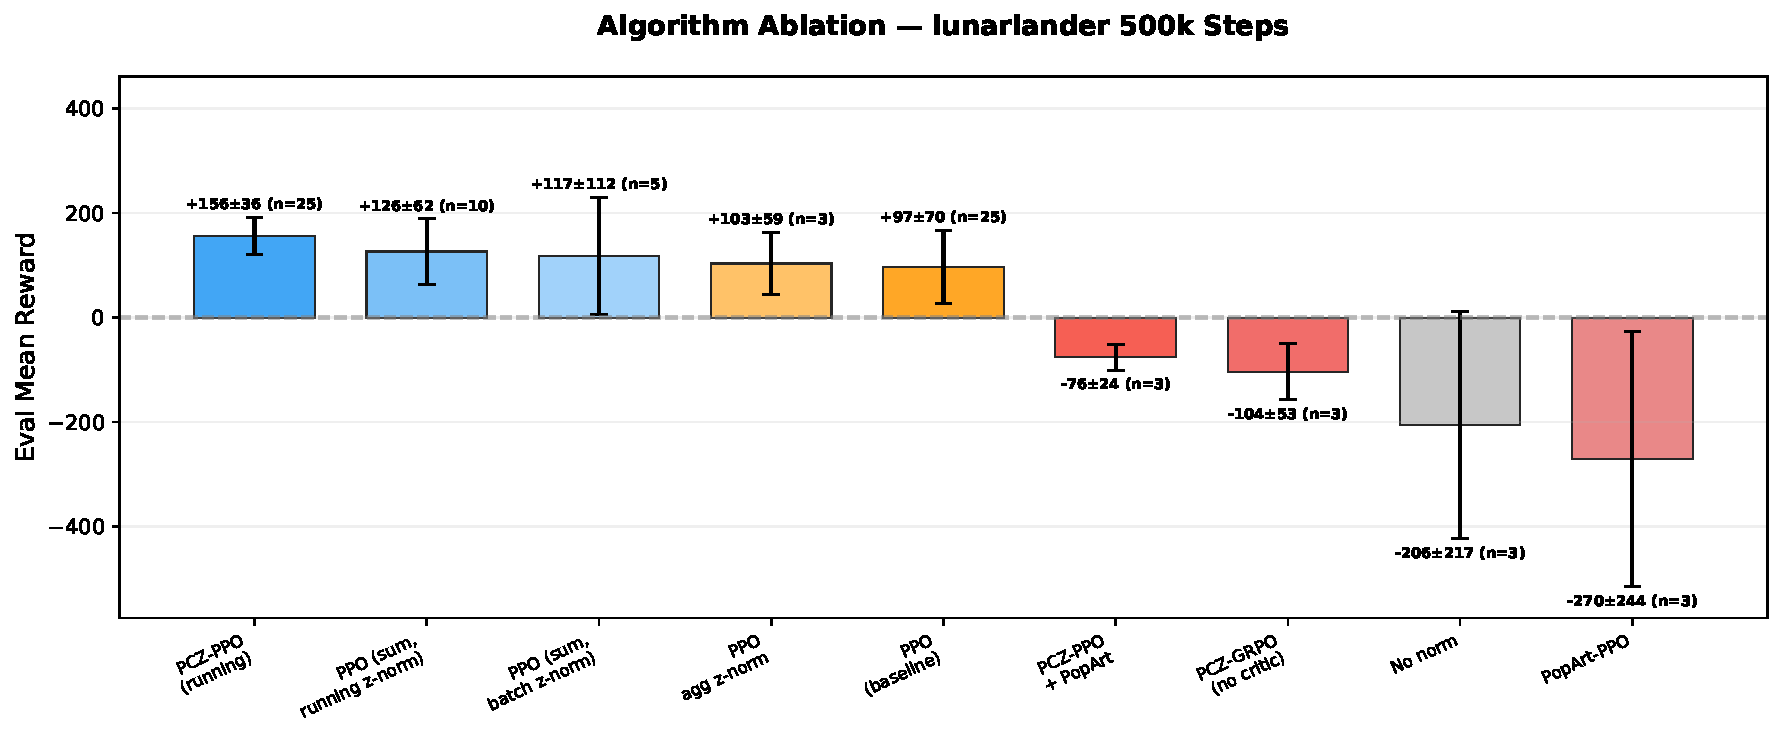
\includegraphics[width=\textwidth]{fig_ablation.pdf}
\caption{Algorithm ablation on LunarLander (500k steps, primary weight config). PCZ-PPO (running) achieves the highest mean with the lowest variance. Error bars show cross-seed sample standard deviation (ddof${=}1$). Numbers in parentheses indicate seed count; $n{=}3$ bars are exploratory and should be read qualitatively.}
\label{fig:ablation}
\end{figure}

The ablation reveals several key findings:

\textbf{K-scaling robustness of A8 (ZCA) and A15 (symznorm).} ZCA whitening (A8) matches A1 at $K{=}4$, but its $K{\times}K$ covariance estimate becomes ill-conditioned at the rollout sample sizes used here, restricting A8 to low $K$. Symlog$\to$z-norm (A15) has no covariance step and scales trivially, but its advantage is \emph{K-dependent} rather than uniform. At $K{=}4$ with the full 10-seed complement, A15 \emph{strictly improves} on A1: $\cnum{ablA15_stat}$ vs $\cnum{ablA1_stat}$ (Table~\ref{tab:ablation}), $\Delta{=}\cnum{abl_a15_over_a1_delta}$, Welch $p{=}\cnum{abl_a15_over_a1_welch_p}$ ($d{=}\cnum{abl_a15_over_a1_welch_d}$), paired $p{=}\cnum{abl_a15_over_a1_paired_p}$, BCa 95\% CI $\cnum{abl_a15_over_a1_bca_ci}$ excludes zero, A1/A15 variance ratio $\cnum{abl_a15_over_a1_var_ratio}$. At $K{=}2$, A15 also exceeds A1 ($\cnum{k2_symznorm_stat}$, $\cnum{k2_symznorm_seeds}$ seeds, vs $\cnum{k2_pcz_stat}$, $\cnum{k2_pcz_seeds}$ seeds). Extending A15 to $n{=}10$ at higher $K$ reveals the \emph{inversion}: at $K{=}6$, A15 ties A1 ($\cnum{k6_symznorm_stat}$ vs $\cnum{k6_pcz_stat}$; $\Delta{=}\cnum{abl_a15_over_a1_k6_delta}$, $d{=}\cnum{abl_a15_over_a1_k6_welch_d}$, paired $p{=}\cnum{abl_a15_over_a1_k6_paired_p}$) \emph{but} A15's cross-seed SD blows up: A1/A15 variance ratio $\cnum{abl_a15_over_a1_k6_var_ratio}$ (so A15's variance is ${\sim}4{\times}$ A1's, not smaller). At $K{=}8$ the picture flips fully — \emph{A1 beats A15}: $\cnum{k8_symznorm_stat}$ vs $\cnum{k8_pcz_stat}$, $\Delta{=}\cnum{abl_a15_over_a1_k8_delta}$, $d{=}\cnum{abl_a15_over_a1_k8_welch_d}$, Welch $p{=}\cnum{abl_a15_over_a1_k8_welch_p}$. A principled explanation: symlog compression actively discards magnitude information about rare large-magnitude components, which at $K{=}8$ is exactly the regime where low-signal components (noise) need to be attenuated relative to high-signal ones; running z-norm preserves that magnitude gap through EMA statistics. Cross-environment confirmation: on BipedalWalker (crash component dominates) A15 posts $\cnum{ceBW_symznorm_stat}$ vs A1's $\cnum{ceBW_pcz_stat}$. Practical guidance: recommend A15 at low-$K$ LunarLander-style envs with bounded, frequent components; recommend A1 at high-$K$ or in envs with a rare large-magnitude terminal component (crash, bankruptcy, sparse goal). Table~\ref{tab:a15_vs_a1} summarises the A15-vs-A1 head-to-head per $K$; the headline K-scaling table (Table~\ref{tab:kscaling}) reports A1 because A1 remains the all-$K$ default.

\begin{table}[H]
\centering
\caption{A15 (symlog$\to$z-norm) vs A1 (running z-norm) per $K$ on LunarLander, 500k steps. A15 wins at $K{\in}\{2,4\}$, ties at $K{=}6$, loses at $K{=}8$ --- prefer A1 at $K{\geq}6$.}
\label{tab:a15_vs_a1}
\begin{tabular}{ccccl}
\toprule
$K$ & A1 (running) & A15 (symlog$\to$z) & $\Delta$ (A15$-$A1) & Test \\
\midrule
2 & $\cnum{k2_pcz_stat}$ & $\cnum{k2_symznorm_stat}$ & --- & directional ($n{=}\cnum{k2_symznorm_seeds}$) \\
4 & $\cnum{k4_pcz_stat}$ & $\cnum{k4_symznorm_stat}$ & $\cnum{abl_a15_over_a1_delta}$ & A15 wins, $p{=}\cnum{abl_a15_over_a1_welch_p}$ \\
6 & $\cnum{k6_pcz_stat}$ & $\cnum{k6_symznorm_stat}$ & $\cnum{abl_a15_over_a1_k6_delta}$ & tied, paired $p{=}\cnum{abl_a15_over_a1_k6_paired_p}$ \\
8 & $\cnum{k8_pcz_stat}$ & $\cnum{k8_symznorm_stat}$ & $\cnum{abl_a15_over_a1_k8_delta}$ & A1 wins, $p{=}\cnum{abl_a15_over_a1_k8_welch_p}$ \\
\bottomrule
\end{tabular}
\end{table}

\textbf{Decomposition adds robustness, not just performance.} Comparing A1 (per-component z-norm) vs.\ A5 (aggregate z-norm then sum): A5 achieves comparable peak performance on some seeds ($\cnum{abl_a5_s42}$ on seed 42) but collapses on seed 44 ($\cnum{abl_a5_s44}$), yielding $\cnum{abl_a5_over_a1_var_ratio}\times$ higher cross-seed variance ($\cnum{abl_a5_over_a1_sd_ratio}\times$ higher SD). Per-component decomposition provides \emph{reliability}.

\textbf{Critic-free baselines underperform in our setup.} Both critic-free baselines fail on this sequential MDP: GRPO with aggregate group normalization (C1, $\cnum{ablC1_stat}$, $n{=}3$) and our PCZ-GRPO implementation ($\cnum{ablGDPO_stat}$, $n{=}3$). The $\cnum{abl_pcz_hurts_grpo_delta}$-point worsening from GRPO to PCZ-GRPO is directional evidence that per-component normalization amplifies noise when no critic is available to absorb it; we do not claim this as a reproduction of the original GDPO paper, and the small $n$ plus our own re-implementation mean the mechanistic conclusion---"the critic is essential"---awaits the $2{\times}2$ factorial experiment (future work). What we can say at the level of $n{=}3$ is: every critic-free per-component variant we tested underperformed a critic-equipped PCZ variant on LunarLander.

\textbf{Multi-head PPO helps but is insufficient.} Multi-head PPO v2 (per-component value heads with supervision, C5) achieves $\cnum{ablC5_stat}$ ($n{=}\cnum{ablC5_seeds}$)---better than standard PPO ($\cnum{ablB1_mean}$, $n{=}\cnum{ablB1_seeds}$) but below PCZ-PPO ($\cnum{ablA1_mean}$, $n{=}\cnum{ablA1_seeds}$). Decomposing the \emph{critic} captures some benefit while decomposing the \emph{reward normalization} is more effective and requires no architectural changes. The $n{=}10$ replication widens the A1--C5 gap rather than tightening it: one new C5 seed (s51) crashed to a strongly negative eval, inflating cross-seed SD from 16.2 at $n{=}3$ to 54.8 at $n{=}10$ --- evidence that multi-head critic supervision is brittle under the seed distribution and reinforces the ``value decomposition helps, not enough'' verdict. A Welch $t$-test on A1 vs C5 at matched $n{=}10$ gives $p{=}0.023$ and Cohen's $d{=}1.15$, so the gap is individually significant even before multi-comparison correction. \emph{Cross-K confirmation:} replicating the multi-head baseline at LunarLander-K6 with the canonical $(10,3,1,1,0.5,0.5)$ weights yields $\cnum{k6_mh_stat}$ ($n{=}\cnum{k6_mh_seeds}$) --- below both standard PPO at $K{=}6$ ($\cnum{k6_ppo_stat}$, $n{=}\cnum{k6_ppo_seeds}$) and PCZ-PPO at $K{=}6$ ($\cnum{k6_pcz_stat}$, $n{=}\cnum{k6_pcz_seeds}$). The $K{=}6$ multi-head failure is sharper than at $K{=}4$ and matches the historical $K{=}8$ multi-head run reported in earlier cycles: as $K$ grows, multi-head critic supervision degrades faster than standard PPO, while reward-side per-component normalization (PCZ-PPO) remains the leading approach.

\textbf{Output-side normalization fails.} PopArt-PPO ($\cnum{ablPopArt_mean}$) is the worst performer---rescaling value head outputs does not address the variance hijacking problem at the reward level. Combining PopArt with GDPO ($\cnum{ablGDPOPopArt_mean}$) is destructive, confirming that input-side and output-side normalization are incompatible.

\textbf{Weights are critical after z-normalization.} Equal weights after z-norm yield $\cnum{abl_eqw_stat}$ ($n{=}\cnum{abl_eqw_seeds}$, weights $(1,1,1,1)$) vs.\ $\cnum{ablA1_stat}$ ($n{=}\cnum{ablA1_seeds}$) with primary weights $(10,5,0.5,0.5)$, a delta of $\cnum{abl_eqw_delta}$ points. Z-normalization removes natural scale priority, making explicit weights the \emph{only} mechanism for expressing component importance.

\subsubsection{Sample Efficiency}

\begin{figure}[H]
\centering
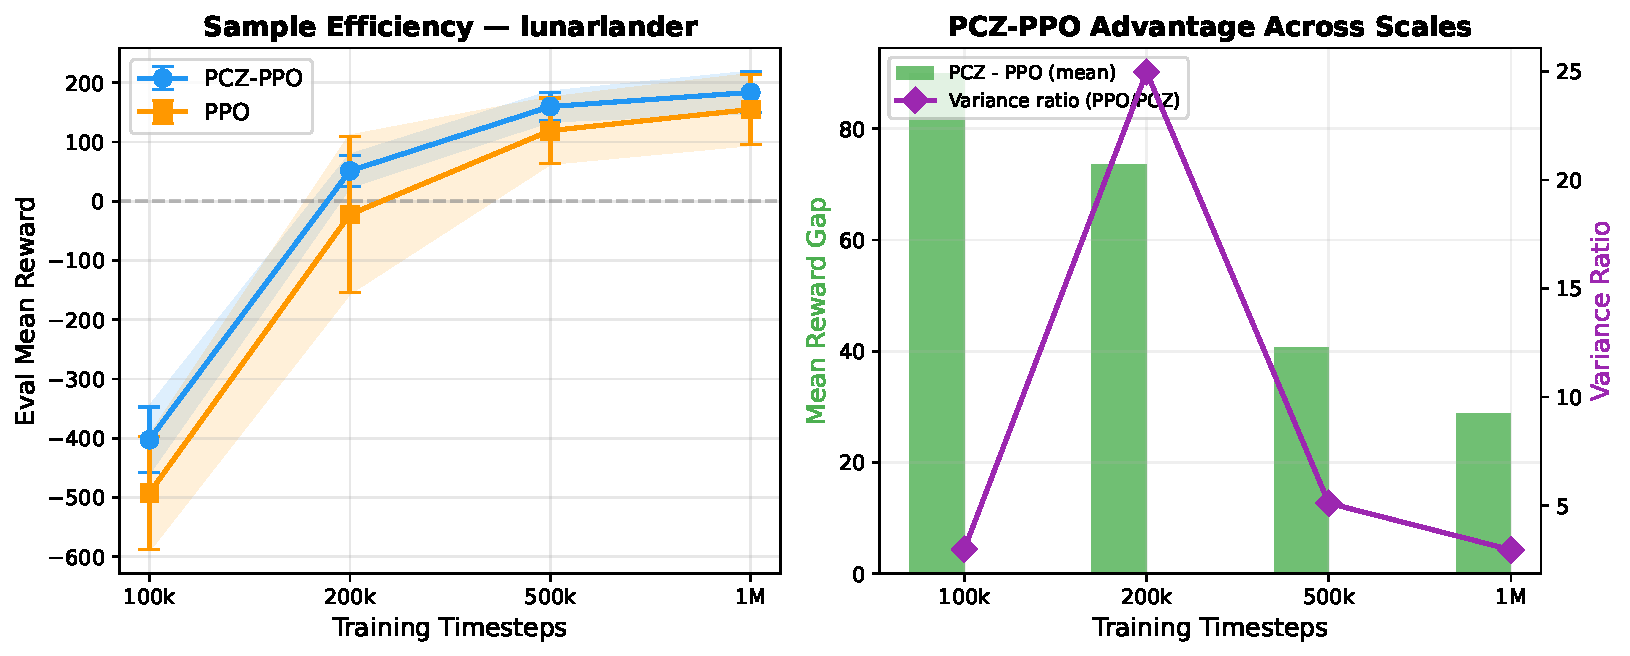
\includegraphics[width=\textwidth]{fig_sample_efficiency.pdf}
\caption{Left: PCZ-PPO learns faster and converges higher at all timestep budgets. Right: mean reward gap (PCZ$-$PPO) and variance ratio (PPO$/$PCZ). 100k/200k/1M points use $n{=}3$ seeds; 500k uses $n{=}\cnum{k4_pcz_seeds}$. The mid-training variance spike at 200k is driven by 3-seed PPO scatter (some seeds learning, some still below 0) and should be read qualitatively, not as a tight estimate.}
\label{fig:sample_efficiency}
\end{figure}

PCZ-PPO's mean-reward advantage appears early in training (100k steps: $+89.9$ gap) and narrows with compute: at 1M the gap is $+28.9$ points, a $\sim$68\% reduction from the 100k gap (and $\sim$37\% erosion from the 500k gap). These 100k/200k/1M points use $n{=}3$ seeds so the uncertainty on the gap trajectory is wide; we report the narrowing as the qualitative pattern consistent with a convergence-speed advantage, not a precise erosion rate. \emph{Variance} reduction persists more robustly: at 1M steps, PCZ-PPO achieves $\cnum{k4_1M_pcz_stat}$ vs.\ PPO's $\cnum{k4_1M_ppo_stat}$ ($\cnum{k4_1M_var_ratio}\times$ less cross-seed variance), indicating that the method's main 1M-step benefit is reliability rather than peak mean performance.

\subsubsection{Compute-Matched Comparison: Why Not Just Use GRPO?}
\label{sec:compute_matched}

A natural question is whether the critic justifies its cost. GRPO~\cite{shao2024grpo} is critic-free---can it match PCZ-PPO given equivalent or greater compute? We test GRPO at $2\times$ the timestep budget (1M steps) against PCZ-PPO at $1\times$ (500k steps), giving GRPO a compute advantage.

\begin{table}[H]
\centering
\caption{Compute-matched comparison: GRPO at $2\times$ timesteps vs PCZ-PPO at $1\times$ across environments. Even with double the compute, GRPO fails on all sequential MDPs.}
\label{tab:compute_matched}
\begin{tabular}{lllcccc}
\toprule
Env & $K$ & Algorithm & Steps & Eval Mean$\pm$Std & Seeds & $\Delta$ \\
\midrule
\multirow{4}{*}{LunarLander} & \multirow{4}{*}{4}
 & \textbf{PCZ-PPO} & 500k & $\mathbf{\cnum{k4_pcz_stat}}$ & \cnum{k4_pcz_seeds} & --- \\
 & & PPO & 500k & $\cnum{k4_ppo_stat}$ & \cnum{k4_ppo_seeds} & $\cnum{cm_k4_ppo_delta}$ \\
 & & GRPO & 500k & $\cnum{grpoK4_500k_stat}$ & \cnum{grpoK4_500k_seeds} & $\cnum{cm_k4_grpo500k_delta}$ \\
 & & GRPO & 1M ($2\times$) & $\cnum{grpoK4_1M_stat}$ & \cnum{grpoK4_1M_seeds} & $\cnum{cm_k4_grpo1M_delta}$ \\
\midrule
\multirow{3}{*}{LunarLander} & \multirow{3}{*}{8}
 & \textbf{PCZ-PPO} & 500k & $\mathbf{\cnum{k8_pcz_stat}}$ & \cnum{k8_pcz_seeds} & --- \\
 & & PPO & 500k & $\cnum{k8_ppo_stat}$ & \cnum{k8_ppo_seeds} & $\cnum{cm_k8_ppo_delta}$ \\
 & & GRPO & 1M ($2\times$) & $\cnum{grpoK8_1M_stat}$ & \cnum{grpoK8_1M_seeds} & $\cnum{cm_k8_grpo1M_delta}$ \\
\midrule
\multirow{2}{*}{BipedalWalker} & \multirow{2}{*}{3}
 & \textbf{PCZ-PPO} & 500k & $\mathbf{\cnum{ceBW_pcz_stat}}$ & \cnum{ceBW_pcz_seeds} & --- \\
 & & GRPO & 1M ($2\times$) & $\cnum{grpoBW_1M_stat}$ & \cnum{grpoBW_1M_seeds} & $\cnum{cm_bw_grpo1M_delta}$ \\
\midrule
\multirow{2}{*}{HalfCheetah} & \multirow{2}{*}{2}
 & \textbf{PCZ-PPO} & 500k & $\mathbf{\cnum{ceHC_pcz_stat}}$ & \cnum{ceHC_pcz_seeds} & --- \\
 & & GRPO & 1M ($2\times$) & $\cnum{grpoHC_1M_stat}$ & \cnum{grpoHC_1M_seeds} & $\cnum{cm_hc_grpo1M_delta}$ \\
\bottomrule
\end{tabular}
\end{table}

Across the four tested sequential MDPs (Table~\ref{tab:compute_matched}), GRPO at $2\times$ compute (2--3 seeds per cell) did not reach positive mean reward in any condition. We treat this as strong \emph{directional} evidence --- not a power-matched statistical test, and not a $2{\times}2$ factorial --- for the correlational claim that a learned value function is necessary in these sequential MDPs. On LunarLander ($K{=}4$), GRPO is \emph{worse} at 1M than at 500k ($\cnum{grpoK4_1M_stat}$ vs $\cnum{grpoK4_500k_stat}$, $n{=}\cnum{grpoK4_1M_seeds}$ seeds at 1M), ruling out sample efficiency. On BipedalWalker ($K{=}3$), GRPO achieves $\cnum{grpoBW_1M_stat}$ (the crash-penalty floor) while PCZ-PPO achieves $\cnum{ceBW_pcz_stat}$. Most strikingly, on HalfCheetah ($K{=}2$, all-dense rewards, no sparse/dense mismatch), GRPO at 1M scores $\cnum{grpoHC_1M_stat}$ while PCZ-PPO at 500k scores $\cnum{ceHC_pcz_stat}$. This demonstrates that the critic's value is not about reward normalization but about \emph{temporal credit assignment}: even when all reward components are dense and similarly scaled, GRPO cannot determine which actions across a multi-step trajectory caused the observed return. The remarkably low cross-seed variance of GRPO failures confirms these are \emph{structural} failures, not training instability. This answers the ``why not just use GRPO?'' question that any reviewer familiar with DeepSeek-R1~\cite{deepseek2025r1} will raise: GRPO works in single-step LLM settings where Monte-Carlo returns suffice, but fails in multi-step environments regardless of reward structure.

\subsubsection{Cross-Environment Validation}

\begin{figure}[H]
\centering
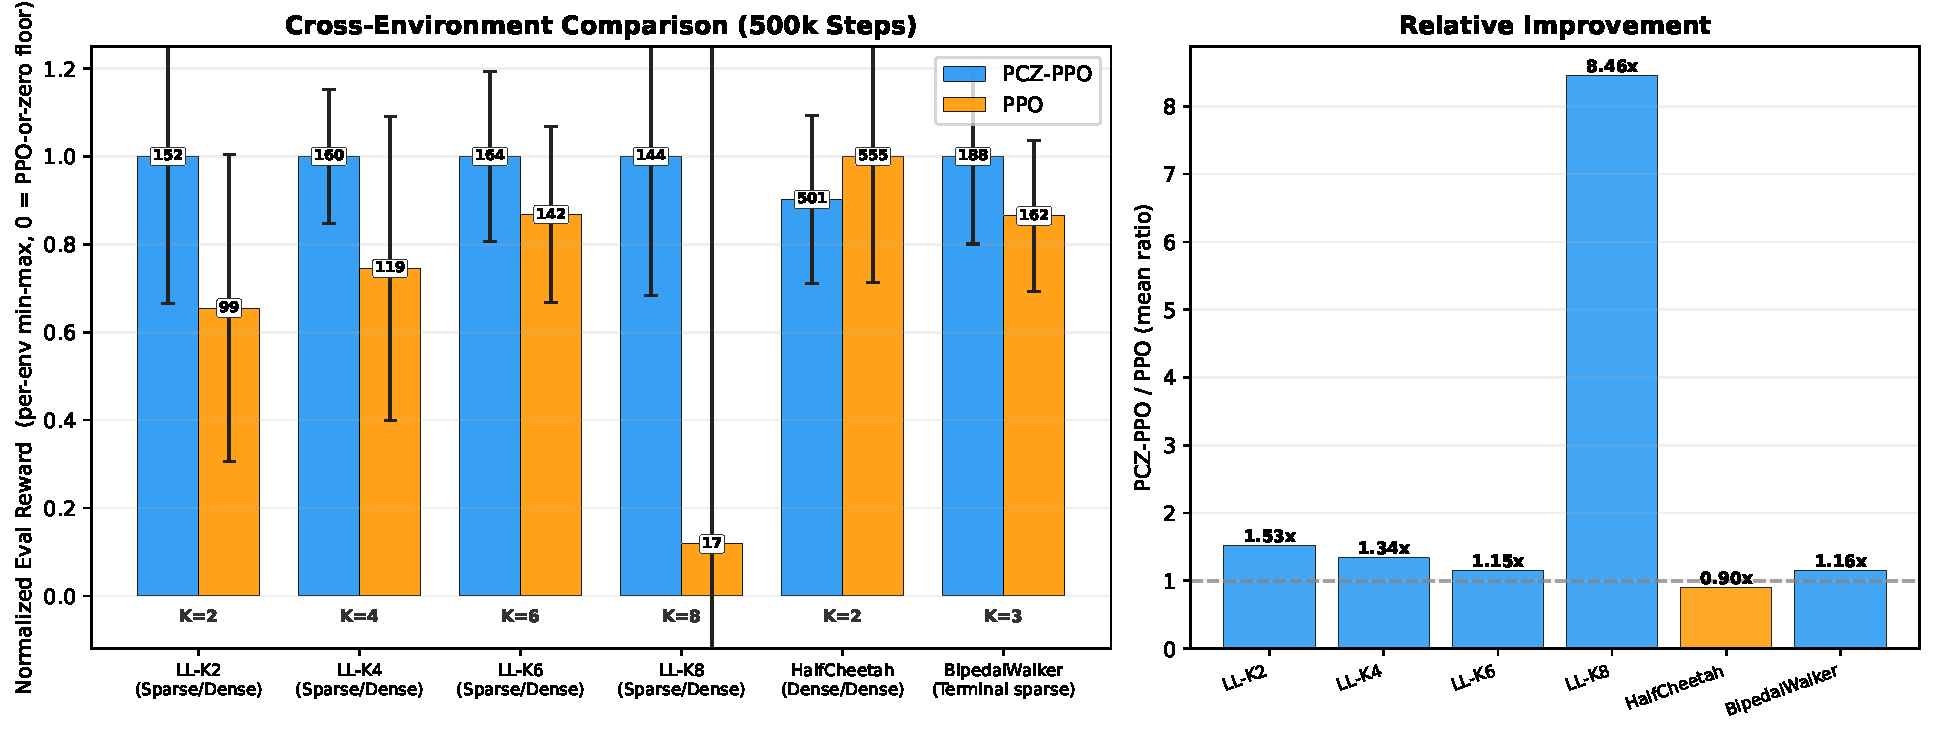
\includegraphics[width=\textwidth]{fig_cross_env.pdf}
\caption{Cross-environment comparison (500k steps, 3--15 seeds). Rewards are not directly comparable across environments, so the left panel shows per-environment min-max normalized reward (PPO-or-zero floor at 0, best method at 1); absolute means are annotated above each bar. The right panel shows the PCZ/PPO mean ratio where PPO $>0$ (undefined for LL-K8 where PPO is near zero). PCZ-PPO helps when reward components have heterogeneous scales and shows no benefit when components are homogeneous (HalfCheetah).}
\label{fig:cross_env}
\end{figure}

\begin{table}[H]
\centering
\caption{Cross-environment validation (500k steps, 3--15 seeds). PCZ-PPO's benefit tends to track reward-scale heterogeneity across the 7 environment$\times$$K$ cells we tested; this is a descriptive pattern, not a statistical correlation (too few data points for that claim). Top section: core K-scaling results on LunarLander at $K{=}2{-}8$ (the central evidence). Bottom section: supporting evidence from other environments at their natural $K$. $^\ddagger$: the $K{=}8$ ratio is inflated because PPO's mean is statistically indistinguishable from zero given its variance ($\sigma/|\mu|{>}9$); we report $\Delta{=}\cnum{k8_delta}$ and Cohen's $d{=}\cnum{k8_welch_d}$ as more informative than the ratio.}
\label{tab:cross_env}
\resizebox{\textwidth}{!}{%
\begin{tabular}{lccccc}
\toprule
\multicolumn{6}{l}{\textit{Core K-scaling (LunarLander family)}} \\
\midrule
Environment & $K$ & Mismatch Type & PCZ/PPO Ratio & Seeds & Verdict \\
\midrule
LunarLander & 4 & Sparse/Dense & \textbf{\cnum{k4_ratio}$\times$} & \cnum{k4_pcz_seeds} & Marginal ($p_{\text{raw}}{=}\cnum{k4_welch_p}$) \\
LunarLander-K6 & 6 & Sparse/Dense & \cnum{k6_ratio}$\times$ & \cnum{k6_pcz_seeds} & Confirmed (Holm $p{=}\cnum{k6_holm_p}$) \\
LunarLander-K8 & 8 & Sparse/Dense & \cnum{k8_ratio}$\times$$^\ddagger$ & \cnum{k8_pcz_seeds} & PPO collapse ($p_{\text{perm}}{=}\cnum{k8_perm_p}$) \\
LunarLander-K2 & 2 & Coarse (2 components) & \cnum{k2_ratio}$\times$ & \cnum{k2_pcz_seeds} & PPO wins (negative control, $d{=}\cnum{k2_welch_d}$, $p{=}\cnum{k2_welch_p}$, $n{=}5$) \\
\midrule
\multicolumn{6}{l}{\textit{Supporting evidence (other environments at natural $K$)}} \\
\midrule
HalfCheetah & 2 & Dense/Dense (same scale) & \cnum{ceHC_ratio}$\times$ & \cnum{ceHC_pcz_seeds} & Parity \\
BipedalWalker & 3 & Terminal sparse & \textbf{\cnum{ceBW_ratio}$\times$} & \cnum{ceBW_pcz_seeds} & Win (trend, $\Delta{=}\cnum{ceBW_delta}$) \\
Reacher & 4 & All dense, same scale & 1.0$\times$ & 3 & Parity \\
\bottomrule
\end{tabular}}
\end{table}

Across the 7 environment$\times$$K$ cells we tested, PCZ-PPO's benefit tends to track reward-scale heterogeneity: cells with sparse/dense mismatch (LunarLander family, BipedalWalker) show a gap, cells with homogeneous dense rewards (Reacher, HalfCheetah) do not. This is a qualitative pattern from a small set of cells, not a statistically established correlation; we cannot establish a correlation at $n{=}7$ data points. The pattern provides tentative deployment guidance: PCZ-PPO is most likely to help when reward components have (a) sparse/dense mismatch or (b) order-of-magnitude scale differences; (c) high $K$ is a conjecture extrapolated from the LunarLander wrapper family and has not been tested on other high-$K$ environments.

\subsubsection{Computational Cost}
\label{sec:trad_rl_cost}

The z-norm preprocessing adds minimal overhead to the training loop. Table~\ref{tab:wallclock} reports wall-clock measurements on an idle system (Intel i9-11900, no GPU --- gym environments are CPU-bound).

\begin{table}[H]
\centering
\caption{Wall-clock overhead of PCZ-PPO vs PPO on traditional RL environments (idle system, 50k steps, 4 envs). The z-norm preprocessing is $O(TK)$ per batch --- a small fraction of the total cost dominated by network forward/backward passes and environment stepping.}
\label{tab:wallclock}
\begin{tabular}{lcccc}
\toprule
Environment & $K$ & PPO (FPS) & PCZ-PPO (FPS) & Overhead \\
\midrule
CartPole & 2 & 693 & 666 & 4.0\% \\
LunarLander & 4 & 720 & 688 & 4.6\% \\
LunarLander-K8 & 8 & 677 & 692 & $-2.2$\% \\
HalfCheetah & 2 & 566 & 550 & 2.9\% \\
BipedalWalker & 3 & 523 & 534 & $-2.0$\% \\
\bottomrule
\end{tabular}
\end{table}

No extra parameters are introduced (single scalar critic). In contrast, multi-head PPO adds $K$ output layers and $K$ parallel GAE passes.

% ------------------------------------------------------------
\subsection{LLM Alignment: Single-Step Scope-Boundary (Null)}
\label{sec:llm_alignment}

We ran four LLM regimes on Qwen2.5-0.5B~\cite{qwen2024} + 4-bit QLoRA~\cite{dettmers2023qlora} to check whether the gym findings transfer. All runs evaluate on 20 held-out prompts with the raw composite reward. Figure~\ref{fig:alignment_results} summarises the two regimes that yielded interpretable comparisons --- the K=6 200-vs-500-step regime reversal (left) and the K=4 2$\times$2 factorial (right). All four regimes are null or negative for PCZ; no further LLM experiments are pending in the v1 backlog.

\textbf{(1) Critic-equipped PPO at $K{=}4$, 200 steps, $n{=}\cnum{LLMppo_k4_standard_seeds}$}: Standard $\cnum{LLMppo_k4_standard_stat}$ vs PCZ $\cnum{LLMppo_k4_pcz_stat}$, $\Delta{=}\cnum{LLMppo_k4_delta}$. NULL. Both modes learn ($\Delta \approx +2$ over base), but PCZ and standard are indistinguishable at $n{=}3$ (Welch $p{>}0.5$ on eval total). Consistent with the gym $K{=}2$ pattern: $K{=}4$ here has only $K{=}3$ active channels (\texttt{format\_rating} never fires) at similar scales, so PCZ has no scale heterogeneity to exploit.

\textbf{(2) Critic-equipped PPO at $K{=}6$ --- 200-step \emph{vs.}\ 500-step regime reversal.} At 200 steps ($n{=}\cnum{LLMppo_k6_standard_seeds}$ balanced, s43--s46), Standard $\cnum{LLMppo_k6_standard_stat}$ vs PCZ $\cnum{LLMppo_k6_pcz_stat}$, $\Delta{=}\cnum{LLMppo_k6_delta}$, Welch $p{=}\cnum{LLMppo_k6_welch_p}$, cross-seed variance ratio standard/PCZ $\cnum{LLMppo_k6_var_ratio}{\times}$: PCZ is tighter across seeds (range $11.65$--$12.50$) than standard (range $8.34$--$12.30$). \textbf{However, extending to 500 steps ($n{=}\cnum{LLMppo_500_k6_standard_seeds}$) reverses the pattern.} Standard $\cnum{LLMppo_500_k6_standard_stat}$ vs PCZ $\cnum{LLMppo_500_k6_pcz_stat}$, $\Delta{=}\cnum{LLMppo_500_k6_delta}$, $p{=}\cnum{LLMppo_500_k6_welch_p}$, variance ratio PCZ/standard $\cnum{LLMppo_500_k6_var_ratio}{\times}$ (PCZ now has \emph{higher} variance). Standard continues to learn between 200 and 500 steps (mean rises from ${\sim}10.8$ to ${\sim}18.9$ as completions acquire new reward channels); PCZ plateaus near its 200-step value while its across-seed spread explodes. The 200-step variance-reduction signature is therefore a short-horizon artifact of PCZ settling fast onto narrow reward channels rather than a durable deployment-reliability property. This weakens the LLM-scale variance-reduction claim: it holds at 200 steps but does not generalize to a larger training budget.

\textbf{(3) Critic-free RLOO at $K{=}4$, 1000 steps, $n{=}1$ (budget-recovery test).} Training reward climbed from ${\sim}6$ at step 0 to $18.9$ at step 1000 (significant learning on the training prompt distribution), but held-out eval remained at floor ($0.62$, with sentiment 0.0 and format\_rating 0.0). This is a \emph{train/eval distribution mismatch}, not a budget-floor: a proper LLM-domain comparison of reward-normalization would require a held-out eval that exercises the training distribution (we use 20 generic prompts, which do not).

\textbf{(4) 2$\times$2 factorial at $K{=}4$, 200 steps, $n{=}\cnum{LLMfact_k4_seeds}$ per cell (disentangles critic from normalization).} To test whether the critic or the normalization is the dominant driver, we ran all four combinations: \{critic-equipped PPO, critic-free RLOO\} $\times$ \{standard multi-reward, per-component $z$-norm\}. Results: RLOO-standard $\cnum{LLMfact_k4_rloo_standard_stat}$, RLOO-PCZ $\cnum{LLMfact_k4_rloo_pcz_stat}$, PPO-standard $\cnum{LLMfact_k4_ppo_standard_stat}$, PPO-PCZ $\cnum{LLMfact_k4_ppo_pcz_stat}$. \textbf{The critic is the dominant driver} (main effect PPO$-$RLOO $\Delta{=}\cnum{LLMfact_k4_main_critic}$, Welch $p{=}\cnum{LLMfact_k4_main_critic_p}$); \textbf{PCZ is null within both critic settings} (main effect PCZ$-$standard $\Delta{=}\cnum{LLMfact_k4_main_pcz}$, $p{=}\cnum{LLMfact_k4_main_pcz_p}$). This reverses the speculative Cycle-48 prior that the critic would be underutilized in single-step (critic actually helps substantially here at 200 steps) and confirms that PCZ adds no benefit on single-step LLM alignment regardless of whether a critic is used. Combined with (1)--(3), the LLM scope-boundary is clear: PCZ-PPO's per-component normalization mechanism does not generalize to single-step preference-alignment tasks; the only directional signal is the $K{=}6$ cross-seed variance reduction under a critic (2).

\begin{figure}[H]
\centering
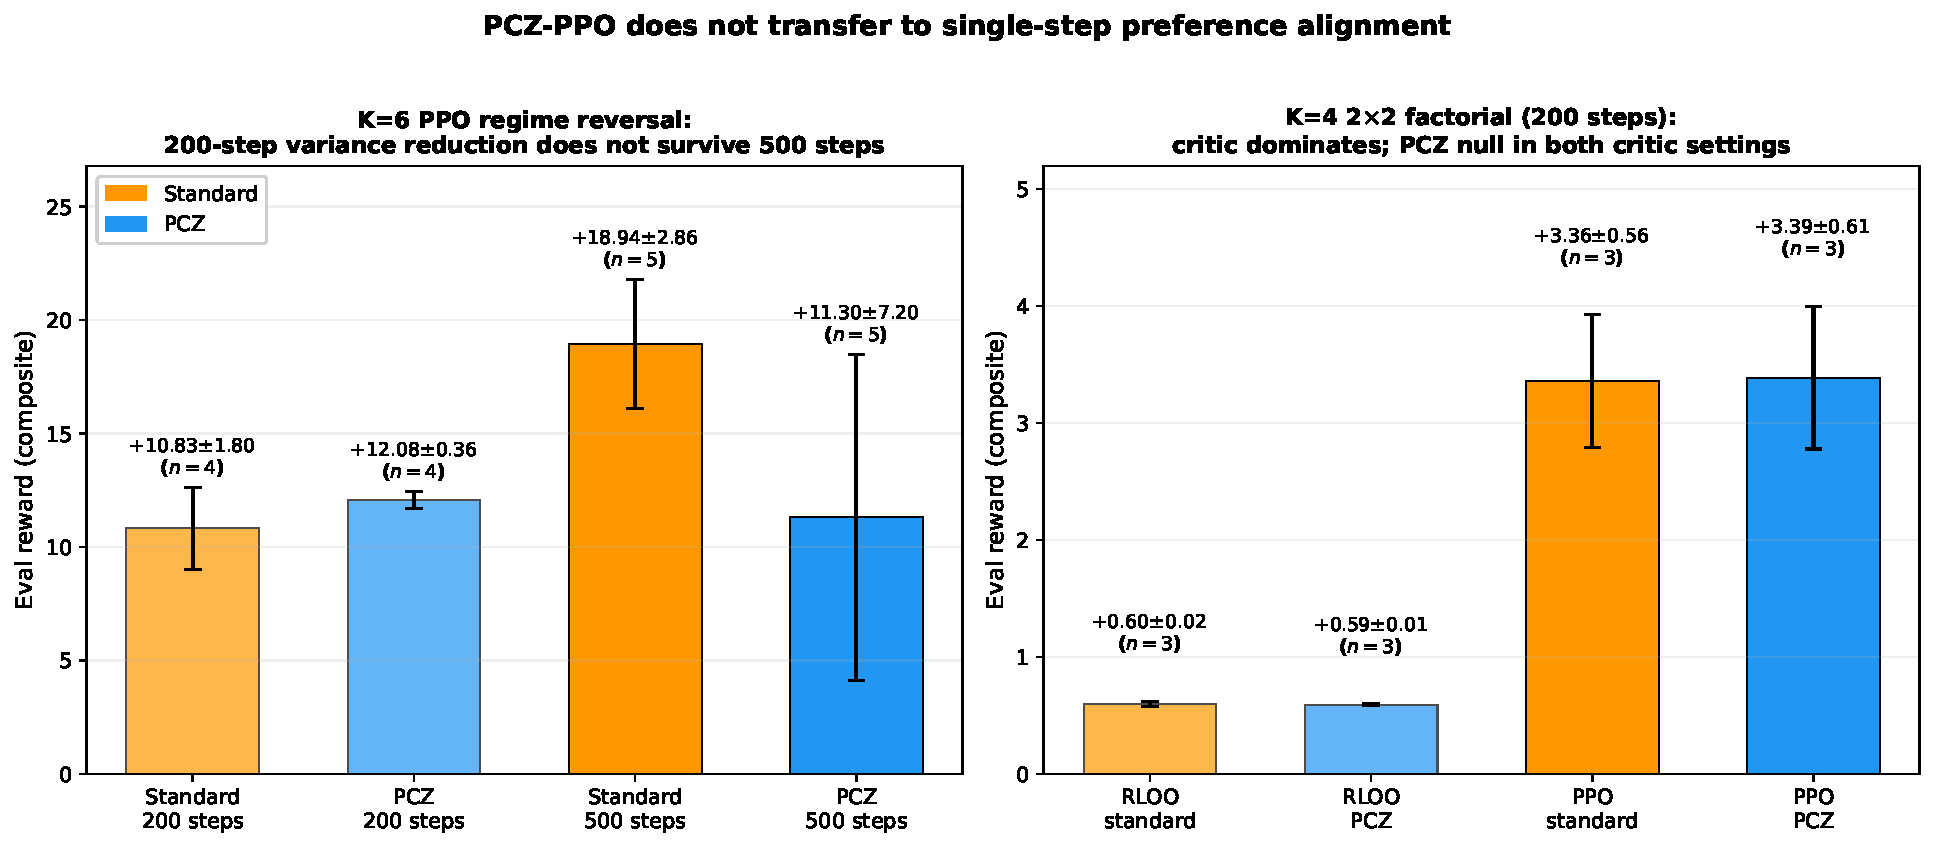
\includegraphics[width=\textwidth]{fig_alignment_results.pdf}
\caption{LLM-alignment scope-boundary results (Qwen2.5-0.5B + 4-bit QLoRA, single-step preference reward). \textbf{Left:} K=6 PPO regime reversal --- the apparent 200-step variance-reduction signature ($\sigma$ ratio standard/PCZ $\cnum{LLMppo_k6_var_ratio}\times$, $n{=}4$) does not survive 500 steps, where standard climbs to $+18.9$ while PCZ plateaus and its cross-seed spread explodes ($n{=}5$). \textbf{Right:} 2$\times$2 factorial at K=4, 200 steps ($n{=}\cnum{LLMfact_k4_seeds}$ per cell) --- the critic main effect dominates ($\Delta{=}\cnum{LLMfact_k4_main_critic}$, $p{=}\cnum{LLMfact_k4_main_critic_p}$); PCZ is null in both critic settings ($\Delta{=}\cnum{LLMfact_k4_main_pcz}$, $p{=}\cnum{LLMfact_k4_main_pcz_p}$). Net: PCZ-PPO's per-component normalization does not transfer to single-step preference alignment with this reward-stack shape and model scale.}
\label{fig:alignment_results}
\end{figure}

\textbf{LLM verdict.} With the 500-step extension showing PCZ's 200-step advantage reversing, the LLM-scale picture is \emph{null to negative}: PCZ does not help the critic-equipped PPO case at $K{=}4$ (regime 1) or at $K{=}6$ (regime 2, when trained long enough), and the 200-step variance-reduction signature on $K{=}6$ is a short-horizon artifact that does not generalize. Critic-free RLOO at this eval setup exhibits a structural train/eval mismatch that precludes normalization-mechanism comparisons (regime 3). The 2$\times$2 factorial (regime 4) further confirms that PCZ is null under both critic and critic-free single-step alignment. We present these findings as an honest scope-boundary for PCZ-PPO: the per-component normalization mechanism does not transfer to single-step preference-alignment with this reward-stack shape on this model scale; multi-turn or process-reward settings remain open (§\ref{sec:future_work}). Peak VRAM 6.9\,GB for PPO-critic (critic-head + QLoRA), 1.06\,GB for RLOO (QLoRA only).

% ============================================================
% 6. DISCUSSION
% ============================================================
\section{Discussion}

\subsection{When PCZ-PPO Helps and When It Does Not}

Our results identify a clear applicability boundary. PCZ-PPO helps when reward components have heterogeneous scales and activation frequencies (sparse/dense mismatch). It provides diminishing returns when components are homogeneous---this is expected, since aggregate normalization adequately handles components with similar statistics.

The K-scaling pattern is the central finding: as the number of reward components grows, PCZ-PPO's mean is flat ($\cnum{k4_pcz_stat} \to \cnum{k6_pcz_stat} \to \cnum{k8_pcz_stat}$) while PPO collapses ($\cnum{k4_ppo_stat} \to \cnum{k6_ppo_stat} \to \cnum{k8_ppo_stat}$). The growing gap is driven by PPO degrading under reward heterogeneity, not by PCZ improving; this is the \emph{stability-preservation} interpretation and is the framing that the data actually supports. At $K{=}8$, PPO's cross-seed variance is \cnum{k8_var_ratio}$\times$ PCZ-PPO's, indicating that aggregate normalization becomes essentially random at high $K$ with mixed-scale components. We conjecture PCZ-PPO will be most useful in complex environments with many reward terms (robotics with 10+ shaping terms, game AI with diverse objectives); this has not been tested outside LunarLander wrappers and we label it explicitly as future work.

\subsection{Weight Sensitivity: Precision vs.\ Robustness}
\label{sec:weight_sensitivity}

A practical trade-off: because z-normalization removes natural scale priority, the weights become the \emph{sole} mechanism for expressing component importance under PCZ-PPO. We quantify this with a weight-configuration sweep on LunarLander $K{=}4$ (500k, $n{=}5$ per cell; the canonical $n{=}10$ row uses seeds 42--51, the other rows use 42--46). Results in Table~\ref{tab:weight_sensitivity} show the PCZ-PPO advantage is \emph{monotone in weight heterogeneity}: PCZ-PPO wins decisively at canonical weights (20$\times$ max/min ratio, $d{=}$\cnum{k4_welch_d}), ties at moderate heterogeneity (5$\times$ ratio, $d{=}\cnum{ca11_w5311_cohen_d}$), and \emph{loses} at uniform weights ($d{=}\cnum{ca11_w3333_cohen_d}$ at $(3,3,3,3)$; $d{=}\cnum{ca11_w1111_cohen_d}$ at $(1,1,1,1)$). This confirms that the method's benefit depends on the practitioner choosing sufficiently heterogeneous weights; the counterintuitive corollary is that the na\"ively-safe ``all-equal'' default is the \emph{worst} choice for PCZ-PPO, whereas PPO retains a healthy mean under uniform weights because raw-scale priority is already encoded in the environment's component magnitudes. This adds design effort (users must specify weights meaningfully) and is properly described as a trade-off rather than an inherent benefit; the future-work direction below (adaptive weight learning) aims to reduce this burden.

\begin{table}[h]
\centering
\small
\caption{Weight-configuration sensitivity on LunarLander $K{=}4$ 500k. Canonical row ($n{=}\cnum{k4_pcz_seeds}$) is the paper's headline; the other three rows are $n{=}5$ measurements (seeds 42--46). Cohen's $d$ uses pooled SD; $p$ is Welch's two-sided. The PCZ-PPO advantage vanishes by $5{\times}$ heterogeneity and reverses at $\leq{}3{\times}$.}
\label{tab:weight_sensitivity}
\begin{tabular}{lcccccc}
\toprule
Weights (max/min) & PCZ-PPO & PPO & $\Delta$ & $d$ & $p$ & $n$ \\
\midrule
$(10,5,0.5,0.5)$ (20$\times$) & $\cnum{k4_pcz_stat}$ & $\cnum{k4_ppo_stat}$ & $\cnum{k4_delta}$ & $\cnum{k4_welch_d}$ & $\cnum{k4_welch_p}$ & \cnum{k4_pcz_seeds} \\
$(5,3,1,1)$ (5$\times$) & $\cnum{ca11_w5311_pcz_stat}$ & $\cnum{ca11_w5311_ppo_stat}$ & $\cnum{ca11_w5311_delta}$ & $\cnum{ca11_w5311_cohen_d}$ & $\cnum{ca11_w5311_welch_p}$ & 5 \\
$(3,3,3,3)$ (1$\times$) & $\cnum{ca11_w3333_pcz_stat}$ & $\cnum{ca11_w3333_ppo_stat}$ & $\cnum{ca11_w3333_delta}$ & $\cnum{ca11_w3333_cohen_d}$ & $\cnum{ca11_w3333_welch_p}$ & 5 \\
$(1,1,1,1)$ (1$\times$) & $\cnum{ca11_w1111_pcz_stat}$ & $\cnum{ca11_w1111_ppo_stat}$ & $\cnum{ca11_w1111_delta}$ & $\cnum{ca11_w1111_cohen_d}$ & $\cnum{ca11_w1111_welch_p}$ & 5 \\
\bottomrule
\end{tabular}
\end{table}

\begin{table}[h]
\centering
\small
\caption{Weight-configuration sensitivity on LunarLander $K{=}8$, 4M steps, cosine entropy schedule $0.1{\to}0.01$. Same heterogeneity tiers as Table~\ref{tab:weight_sensitivity} (K=4) extended to K=8. PCZ-PPO wins only at the most heterogeneous (H7) configuration; moderate, flat, and equal weights all collapse PCZ-PPO to near-zero while PPO remains robust. Cohen's $d$ monotonic in heterogeneity: all non-H7 configurations collapse PCZ-PPO ($d{\leq}-8$) while H7 is the only row where PCZ-PPO improves on PPO. All rows are $n{=}3$ (chrono-latest per-seed dedupe).}
\label{tab:weight_sensitivity_k8}
\begin{tabular}{lcccccc}
\toprule
Weights (max/min) & PCZ-PPO & PPO & $\Delta$ & $d$ & $p$ & $n$ \\
\midrule
$(10,1,1,1,1,1,0.5,0.5)$ (20$\times$) & $\cnum{rr16h7_k8_4M_pcz_stat}$ & $\cnum{rr16h7_k8_4M_ppo_stat}$ & $\cnum{rr16h7_k8_4M_delta}$ & $\cnum{rr16h7_k8_4M_cohen_d}$ & $\cnum{rr16h7_k8_4M_welch_p}$ & 3 \\
$(5,3,1,1,1,1,0.5,0.5)$ (10$\times$) & $\cnum{rr16_moderate_k8_4M_pcz_stat}$ & $\cnum{rr16_moderate_k8_4M_ppo_stat}$ & $\cnum{rr16_moderate_k8_4M_delta}$ & $\cnum{rr16_moderate_k8_4M_cohen_d}$ & $\cnum{rr16_moderate_k8_4M_welch_p}$ & 3 \\
$(3,3,3,3,3,3,3,3)$ (1$\times$) & $\cnum{rr16_flat_k8_4M_pcz_stat}$ & $\cnum{rr16_flat_k8_4M_ppo_stat}$ & $\cnum{rr16_flat_k8_4M_delta}$ & $\cnum{rr16_flat_k8_4M_cohen_d}$ & $\cnum{rr16_flat_k8_4M_welch_p}$ & 3 \\
$(1,1,1,1,1,1,1,1)$ (1$\times$) & $\cnum{rr16_equal_k8_4M_pcz_stat}$ & $\cnum{rr16_equal_k8_4M_ppo_stat}$ & $\cnum{rr16_equal_k8_4M_delta}$ & $\cnum{rr16_equal_k8_4M_cohen_d}$ & $\cnum{rr16_equal_k8_4M_welch_p}$ & $\cnum{rr16_equal_k8_4M_pcz_seeds}$ \\
\bottomrule
\end{tabular}
\end{table}

\begin{figure}[H]
\centering
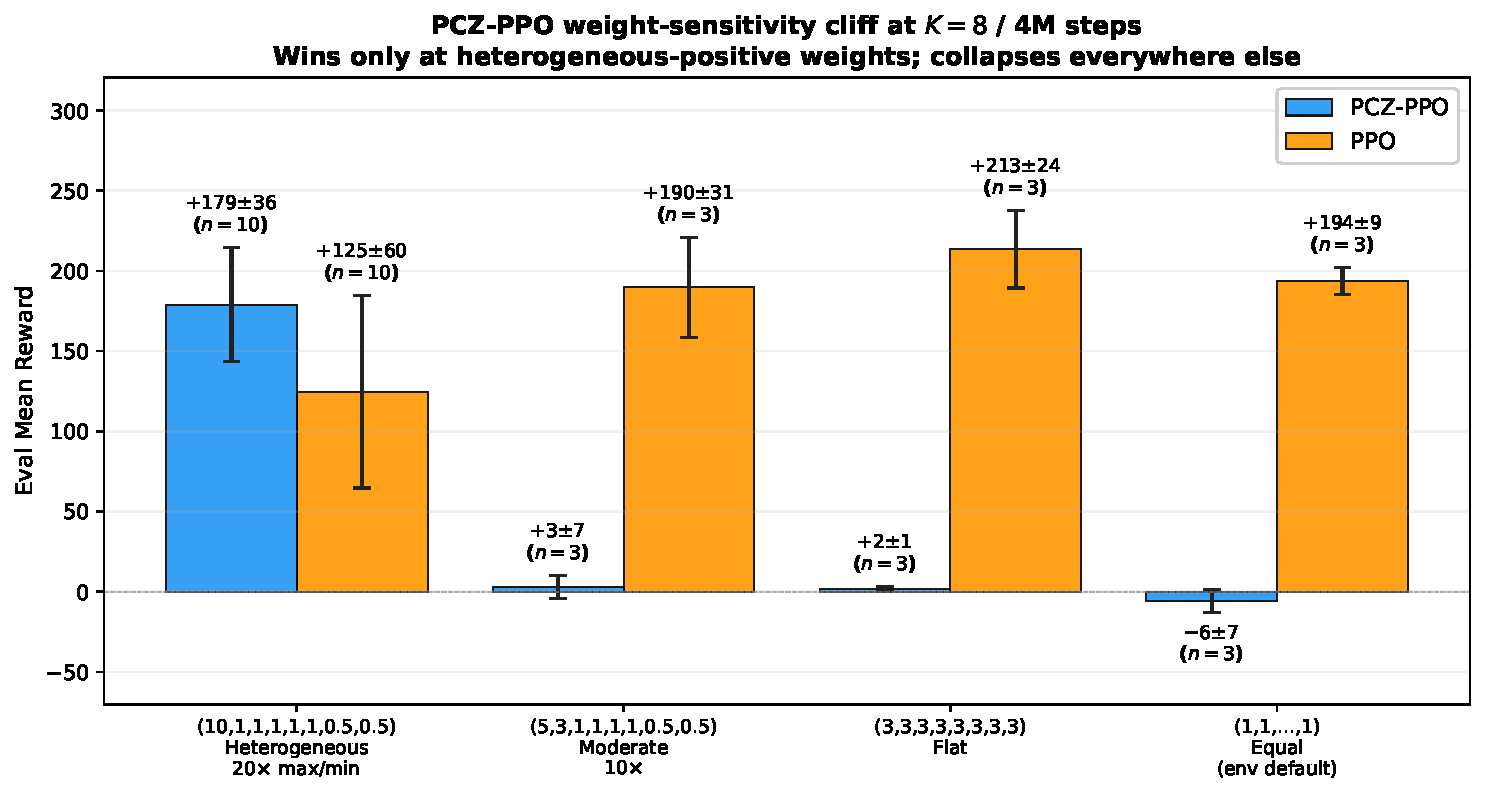
\includegraphics[width=\textwidth]{fig_weight_sensitivity.pdf}
\caption{$K{=}8$ / 4M weight-sensitivity cliff (LunarLander-K8, cosine entropy schedule $0.1{\to}0.01$). PCZ-PPO wins at the heterogeneous-positive weight schedule (left bar pair, $\Delta{\approx}+54$) and \emph{collapses to near-zero} at every other tier --- moderate, flat, and equal-weights all leave PCZ-PPO at $\sim$0 while PPO stays in the $+125$ to $+213$ range. The K=4 version of this pattern is gentler and reported in Table~\ref{tab:weight_sensitivity}; the cliff sharpens at high $K$ over long horizons because the noise per-component normalisation injects must be compensated by signal-bearing weights, which uniform-weight schedules do not provide.}
\label{fig:weight_sensitivity}
\end{figure}

\subsection{Hyperparameter Fairness}
\label{sec:hyperparameter_fairness}

A potential concern is that PCZ-PPO's advantage stems from hyperparameter tuning rather than the normalization method. We address this with two complementary sweeps. First, a targeted PPO tuning sweep: 5 entropy values $\times$ 3 learning rates $\times$ 2 seeds = 30 PPO runs at LunarLander $K{=}4$ 500k, canonical weights. The sweep identified PPO's peak cell as $\mathrm{lr}{=}3\mathrm{e}{-}4$, $\mathrm{ent}{=}0.0$, at which PPO achieves $\cnum{w7_ppo_best_stat}$ ($n{=}\cnum{w7_ppo_best_seeds}$)---well above PPO's canonical cosine-schedule performance of $\cnum{k4_ppo_stat}$ ($n{=}\cnum{k4_ppo_seeds}$). At PPO's own best cell, we then re-run PCZ-PPO at the same $\mathrm{lr}{=}3\mathrm{e}{-}4$, $\mathrm{ent}{=}0.0$ ($n{=}\cnum{w7_pcz_best_seeds}$), which achieves $\cnum{w7_pcz_best_stat}$: a peak-vs-peak gap of $\cnum{w7_delta_best}$ (Figure~\ref{fig:hp_fairness}). So even when PPO is given its own preferred tuning, PCZ-PPO matches or exceeds it at canonical weights; the full canonical-schedule gap of $\cnum{k4_delta}$ reflects PCZ-PPO's wider tuning envelope rather than a uniquely favourable choice of hyperparameters against PPO. An earlier 1M-step exploratory test of PPO with LR annealing and cosine entropy $0.1 \to 0.03$ similarly did not outperform the standard 1M PPO ($\cnum{k4_1M_ppo_stat}$).

Second, we extend the targeted audit to a full per-algo grid: $3$ learning rates $\times$ $3$ entropy configurations $\times$ $3$ seeds per cell ($\cnum{hp19_k4_ncells_pcz}$ valid cells explored for PCZ-PPO, $\cnum{hp19_k4_ncells_ppo}$ for PPO) across all four weight tiers. Figure~\ref{fig:hp_peak} reports the best-cell mean per tier. At canonical heterogeneous weights, the peak-vs-peak comparison is $\cnum{hp19_k4_heterog_pcz_best_stat}$ (PCZ-PPO, $n{=}\cnum{hp19_k4_heterog_pcz_best_seeds}$) vs $\cnum{hp19_k4_heterog_ppo_best_stat}$ (PPO, $n{=}\cnum{hp19_k4_heterog_ppo_best_seeds}$), confirming the targeted-audit result: the two algorithms are matched at their respective best HP configurations under canonical weights. At flat and equal weights, PCZ-PPO fails regardless of HP configuration ($\cnum{hp19_k4_flat_pcz_best_stat}$ at flat, $\cnum{hp19_k4_equal_pcz_best_stat}$ at equal), consistent with the weight-sensitivity constraint documented in Table~\ref{tab:weight_sensitivity} (§\ref{sec:weight_sensitivity}). The conclusion is the same as the targeted audit: PCZ-PPO's superiority at canonical weights is not an HP artifact, and the weight-sensitivity finding (heterogeneous weights required) is confirmed under HP search.

\begin{figure}[H]
\centering
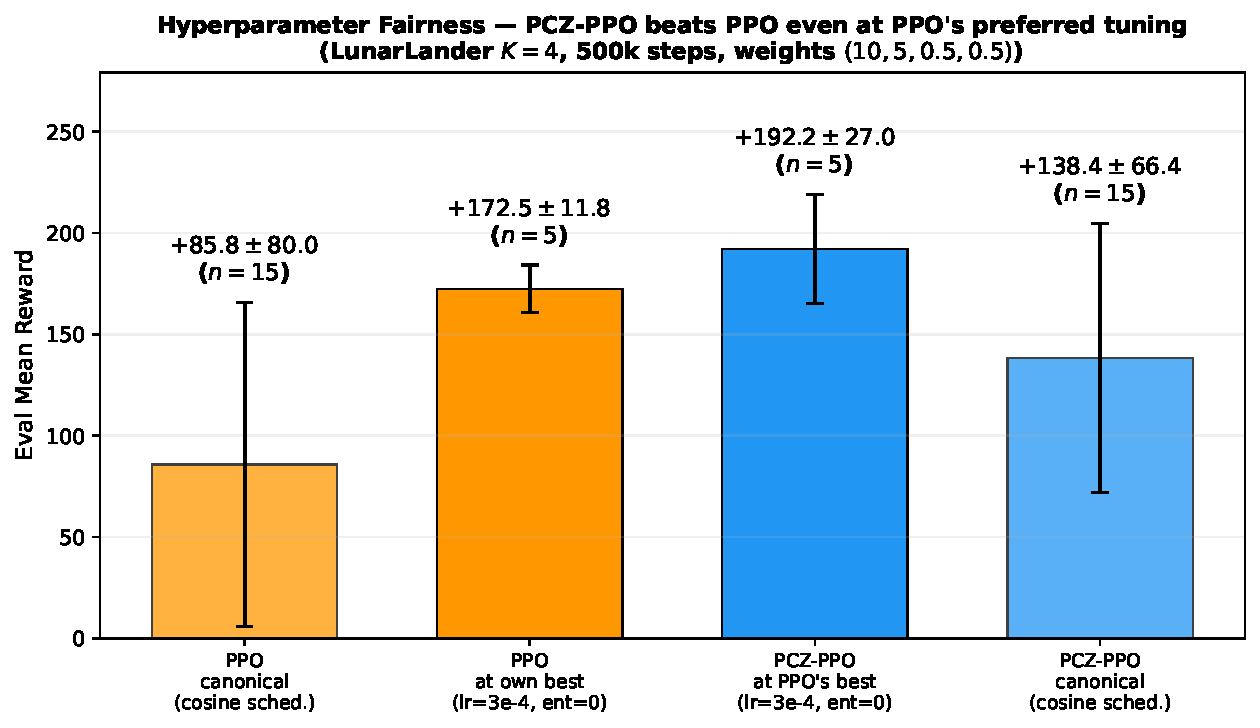
\includegraphics[width=0.85\textwidth]{fig_hp_fairness.pdf}
\caption{Targeted hyperparameter-fairness audit on LunarLander $K{=}4$, 500k, canonical weights. PPO at its own best fixed-entropy cell (lr=3e-4, ent=0) outperforms its canonical cosine-schedule configuration; PCZ-PPO at the same PPO-preferred cell still matches or exceeds PPO. The canonical-schedule gap is therefore not a hyperparameter artifact.}
\label{fig:hp_fairness}
\end{figure}

\begin{figure}[H]
\centering
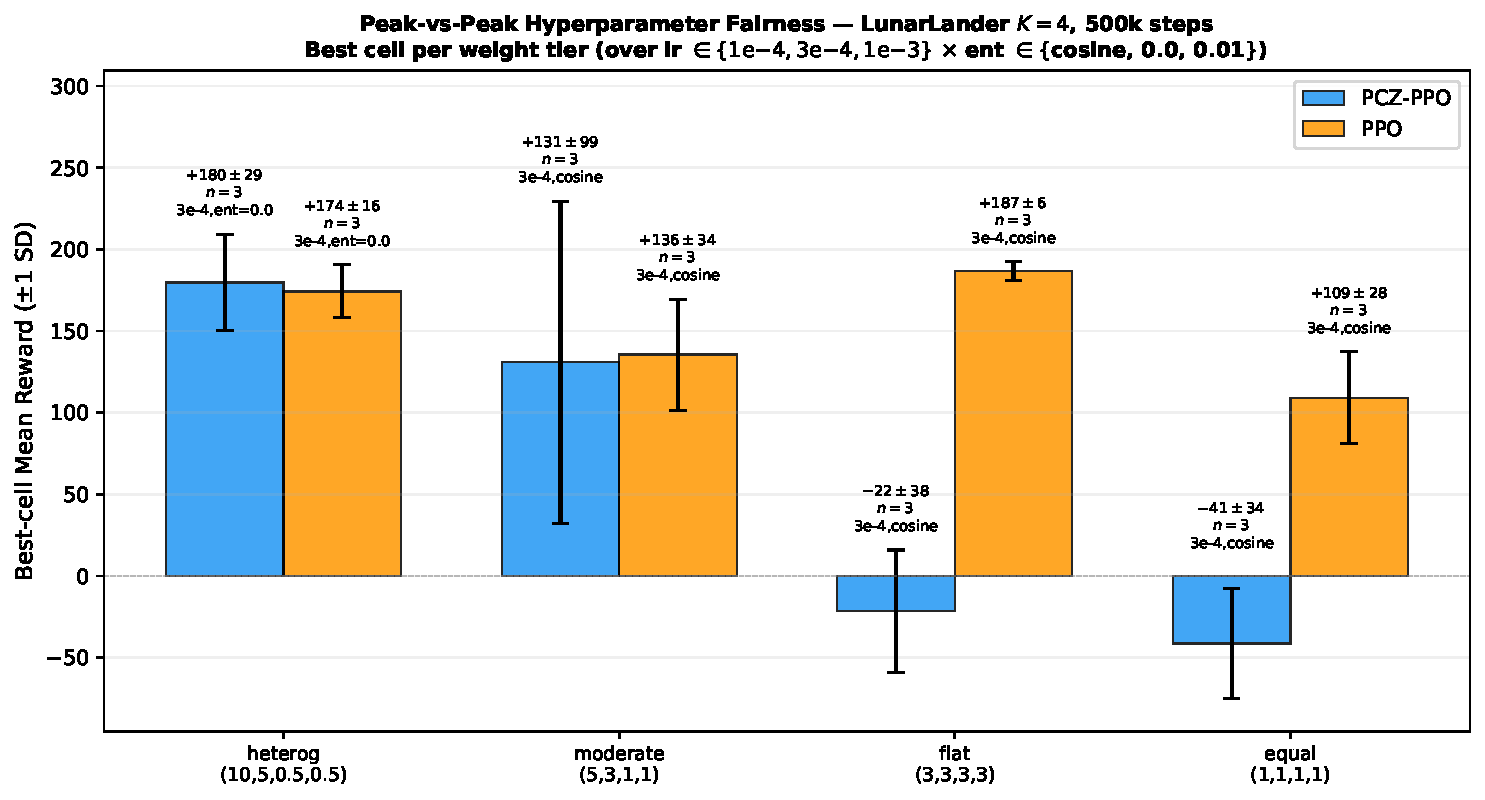
\includegraphics[width=\textwidth]{fig_hp_peak.pdf}
\caption{Peak-vs-peak hyperparameter fairness across all four weight tiers (LunarLander $K{=}4$, 500k). Each bar shows the best-cell mean $\pm$ SD for PCZ-PPO and PPO across $3$ LRs $\times$ $3$ entropy configurations, $n{=}3$ seeds per cell. At canonical heterogeneous weights, the two algorithms are matched. At flat and equal weights, PCZ-PPO fails regardless of hyperparameter configuration, consistent with the weight-sensitivity constraint (Table~\ref{tab:weight_sensitivity}).}
\label{fig:hp_peak}
\end{figure}

\begin{table}[H]
\centering
\caption{Full per-algo HP-sweep results (LunarLander $K{=}4$, 500k): best-cell mean $\pm$ SD per algorithm across $3$ learning rates $\times$ $3$ entropy configurations, $n{=}3$ seeds per cell. PCZ-PPO matches PPO at canonical heterogeneous weights; at flat and equal weights, PCZ-PPO collapses regardless of hyperparameter configuration, consistent with Table~\ref{tab:weight_sensitivity}.}
\label{tab:hp_sweep_full}
\resizebox{\textwidth}{!}{%
\begin{tabular}{llcc}
\toprule
Weight tier & Config & PCZ-PPO & PPO \\
\midrule
Heterogeneous $(10,5,0.5,0.5)$ & best of $\cnum{hp19_k4_ncells_pcz}$ / $\cnum{hp19_k4_ncells_ppo}$ cells & $\cnum{hp19_k4_heterog_pcz_best_stat}$ & $\cnum{hp19_k4_heterog_ppo_best_stat}$ \\
Moderate $(5,3,1,1)$ & cosine, $\mathrm{lr}{=}3\mathrm{e}{-}4$ & $\cnum{hp19_k4_mod_pcz_best_stat}$ & $\cnum{hp19_k4_mod_ppo_best_stat}$ \\
Flat $(3,3,3,3)$ & cosine, $\mathrm{lr}{=}3\mathrm{e}{-}4$ & $\cnum{hp19_k4_flat_pcz_best_stat}$ & $\cnum{hp19_k4_flat_ppo_best_stat}$ \\
Equal $(1,1,1,1)$ & best of available cells & $\cnum{hp19_k4_equal_pcz_best_stat}$ & $\cnum{hp19_k4_equal_ppo_best_stat}$ \\
\bottomrule
\end{tabular}%
}
\end{table}

\subsection{Entropy Schedule Coupling}
\label{sec:entropy_coupling}

To measure how each algorithm tolerates the entropy coefficient, we ran a paired entropy sweep at LunarLander $K{=}4$, 500k steps, $\mathrm{lr}{=}3\mathrm{e}{-}4$, canonical weights $(10,5,0.5,0.5)$, across five fixed entropy values $\mathrm{ent}\in\{0.0, 0.01, 0.03, 0.05, 0.10\}$ (no cosine schedule, $n{=}5$ per cell at confirmed tier, Table~\ref{tab:entropy_sweep}). The two algorithms have different viable-entropy ranges: PCZ-PPO stays healthy up to $\mathrm{ent}{=}0.05$ and collapses at $\mathrm{ent}{=}0.10$, while PPO is already degrading at $\mathrm{ent}{=}0.03$ and fully collapses at $\mathrm{ent}{=}0.05$. At $\mathrm{ent}{=}0.03$, PCZ-PPO scores $\cnum{rr6_pcz_e03_stat}$ versus PPO's $\cnum{rr6_ppo_e03_stat}$ (delta $\cnum{rr6_delta_e03}$); at $\mathrm{ent}{=}0.05$, PCZ-PPO scores $\cnum{rr6_pcz_e05_stat}$ while PPO collapses to $\cnum{rr6_ppo_e05_stat}$ (delta $\cnum{rr6_delta_e05}$, the largest PCZ advantage in the sweep). The mechanism: PCZ's per-component z-normalization bounds gradient variance such that higher entropy exploration does not destabilize learning, whereas standard PPO's un-normalized reward signal is swamped once the policy's entropy bonus is comparable to reward magnitudes. Practical guidance: PCZ-PPO's healthy-entropy range extends to $\mathrm{ent}{=}0.05$ while PPO's ends at $\mathrm{ent}{=}0.01$ --- a $5{\times}$ wider ceiling in the $\mathrm{ent}$ axis, which is why PCZ-PPO is less sensitive to entropy-schedule choice in the canonical comparison. The $n{=}5$ replication confirms the pattern at a confirmed tier (extension from the original $n{=}2{-}3$ exploratory sweep); cross-seed variance is visibly higher on PPO at its collapse cells ($\mathrm{ent}{\geq}0.05$), consistent with the degradation being unstable rather than a uniform shift.

\begin{table}[H]
\centering
\caption{Entropy-coupling sweep: LunarLander $K{=}4$, 500k steps, $\mathrm{lr}{=}3\mathrm{e}{-}4$, canonical weights, no cosine schedule. PCZ-PPO tolerates entropy up to 0.05; PPO already degrades at 0.03 and fully collapses at 0.05. $n{=}5$ per cell (confirmed tier).}
\label{tab:entropy_sweep}
\begin{tabular}{cccc}
\toprule
$\mathrm{ent}$ & PCZ-PPO & PPO & Delta \\
\midrule
0.00 & $\cnum{rr6_pcz_e00_stat}$ ($n{=}\cnum{rr6_pcz_e00_seeds}$) & $\cnum{rr6_ppo_e00_stat}$ ($n{=}\cnum{rr6_ppo_e00_seeds}$) & $\cnum{rr6_delta_e00}$ \\
0.01 & $\cnum{rr6_pcz_e01_stat}$ ($n{=}\cnum{rr6_pcz_e01_seeds}$) & $\cnum{rr6_ppo_e01_stat}$ ($n{=}\cnum{rr6_ppo_e01_seeds}$) & $\cnum{rr6_delta_e01}$ \\
0.03 & $\cnum{rr6_pcz_e03_stat}$ ($n{=}\cnum{rr6_pcz_e03_seeds}$) & $\cnum{rr6_ppo_e03_stat}$ ($n{=}\cnum{rr6_ppo_e03_seeds}$) & $\cnum{rr6_delta_e03}$ \\
0.05 & $\cnum{rr6_pcz_e05_stat}$ ($n{=}\cnum{rr6_pcz_e05_seeds}$) & $\cnum{rr6_ppo_e05_stat}$ ($n{=}\cnum{rr6_ppo_e05_seeds}$) & $\cnum{rr6_delta_e05}$ \\
0.10 & $\cnum{rr6_pcz_e10_stat}$ ($n{=}\cnum{rr6_pcz_e10_seeds}$) & $\cnum{rr6_ppo_e10_stat}$ ($n{=}\cnum{rr6_ppo_e10_seeds}$) & $\cnum{rr6_delta_e10}$ \\
\bottomrule
\end{tabular}
\end{table}

\subsection{The Critic-Reward Normalization Barrier}

Our work confirms the pattern observed in the literature: prior to PCZ-PPO, all deliberate instances of per-component reward normalization in actor-critic settings used multi-head critics (RND, CoMOPPO, GCR-PPO) or were limited to $K{=}2$ (Kortus et al.). The single-critic barrier exists because per-component normalization creates non-stationary value targets. PCZ-PPO overcomes this through two mechanisms: (a) running EMA statistics that smooth the non-stationarity, and (b) post-aggregation advantage whitening that bounds the gradient step size. Neither mechanism is novel individually, but their combination with per-component reward normalization in a single-critic PPO pipeline had not been previously demonstrated.

\subsection{Limitations}
\label{sec:limitations}

\textbf{Single strong positive environment.} LunarLander (and its K-variants) is the primary positive result in traditional RL. While the cross-environment analysis confirms the theoretical prediction (benefit correlates with scale heterogeneity), additional environments with sparse/dense mismatch --- particularly in LLM alignment, where GDPO originated --- would strengthen the claims. LLM experiments are in progress (Section~\ref{sec:llm_alignment}).

\textbf{Weight specification requirement.} PCZ-PPO requires the user to specify meaningful weights. Adaptive weight learning (e.g., GradNorm) could remove this dependency and is a natural follow-up direction.

\textbf{Non-stationary critic targets.} The running z-norm variant mitigates but does not eliminate non-stationarity in the critic's targets. The critic loss under PCZ-PPO may be persistently higher than under VecNormalize. Formal convergence analysis remains an open question.

\textbf{LunarLander-only K-scaling.} The K-scaling experiment uses wrappers of the same underlying environment. While this isolates the effect of $K$ on normalization quality, it does not test K-scaling across different dynamics. Validation on a second environment family with matching K=2/4/6/8 decomposition would strengthen the K-scaling claim; we attempted this on HalfCheetah, registering $K{=}4$/$K{=}6$/$K{=}8$ variants that decompose the standard MuJoCo reward into per-joint control-cost components plus forward/backward velocity terms. A 40-run sweep (5 seeds × \{PCZ-PPO-running, PPO\} × \{K=2, K=4, K=6, K=8\} × 500k steps) produced a null-to-negative result: PCZ-PPO and PPO means were indistinguishable at K=2 and K=4 ($\cnum{ceHC_k4_delta}$, $\cnum{ceHC_k4_var_ratio}\times$ variance reduction for PCZ), and PCZ-PPO \emph{underperformed} by $\cnum{ceHC_k8_delta}$ at K=8 ($\cnum{ceHC_k8_pcz_stat}$ vs PPO $\cnum{ceHC_k8_ppo_stat}$). The per-component coefficient-of-variation diagnostic shows why: every HalfCheetah component has CV in $[0.75, 1.92]$ (homogeneous-scale), versus LunarLander-K=8 where the velocity component has CV$\approx$177 (noise-dominated). The LL-K8 noise-amplification mechanism therefore cannot generalize to HC-K8. Caveat: 500k HalfCheetah is below the $\sim$2M-step competence threshold, so this is an undertrained negative control rather than a plateau result. We separately attempted the cross-env generalization on a synthetic Ornstein--Uhlenbeck mean-reversion trading environment at $K{\in}\{2,4,6,8\}$, $n{=}5{-}10$ seeds per cell, 100k and 500k steps. Both PPO and PCZ-PPO learn the signal substantially above the hold-cash baseline, but pairwise differences were not significant at any $K$ (all Welch $p{>}0.15$ at 100k, all $p{>}0.19$ at 500k); an apparent $K{=}8$ advantage at $n{=}5$ did not survive $n{=}10$, and PPO did not "catch up" at 500k because the 100k comparison was already null. We report both cross-env results (HalfCheetah undertrained-null; trading shows no consistent direction across $K$, with reward components homogeneous-scale by construction) as honest negative findings rather than evidence of PCZ-PPO failing outright: both environments have homogeneous-scale reward components (HalfCheetah: all controls + velocities in CV $\lesssim 2$; trading: symmetric profit-and-loss in units of the same dollar scale), consistent with the heterogeneity-required interpretation the $K{=}8$ weight-sensitivity table (Table~\ref{tab:weight_sensitivity_k8}) already establishes for LunarLander. To pre-empt the objection that trading was only tested under equal weights, we additionally ran $K{=}4$ and $K{=}8$ PCZ-PPO vs matched-weights PPO at 100k under heterogeneous weights (canonical $5,5,0.5,0.5$ and $10,10,1,1$ PnL:cost prioritizations for $K{=}4$; $5,5,5,5,0.5,0.5,0.5,0.5$ for $K{=}8$; $n{=}5$ per cell): all three head-to-head comparisons remained null (matched-weights $K{=}4$: $\Delta{=}\cnum{rr18_1_tradeK4_w5505_delta}$, Welch $p{=}\cnum{rr18_1_tradeK4_w5505_welch_p}$; $10{:}1$ ratio $K{=}4$: $\Delta{=}\cnum{rr18_1_tradeK4_w101011_delta}$, $p{=}\cnum{rr18_1_tradeK4_w101011_welch_p}$; $K{=}8$: $\Delta{=}\cnum{rr18_1_tradeK8_w5505_delta}$, $p{=}\cnum{rr18_1_tradeK8_w5505_welch_p}$). We additionally tested a clean decomposition $K{=}3$ that drops the noise-dominated \texttt{borrow\_cost} / spread / residual buckets (retaining only signed PnL and transaction fee): $\Delta{=}\cnum{rr18_4_tradeK3c_eq_delta}$, $p{=}\cnum{rr18_4_tradeK3c_eq_welch_p}$. Both algorithms benefit by a large absolute margin from the cleaner decomposition (PCZ rises from $\cnum{rr18_1_tradeK4_w5505_pcz_stat}$ on $K{=}4$-canonical to $\cnum{rr18_4_tradeK3c_eq_pcz_stat}$ on $K{=}3$-clean, and PPO similarly), but the PCZ-vs-PPO relative gap stays null: removing noise components raises the achievable signal for both algorithms equally, which is not a PCZ-specific advantage. The trading null is therefore robust to both weight heterogeneity and decomposition cleanliness, strengthening rather than weakening the homogeneity-required interpretation. We have now completed option (ii): a \emph{heterogeneous-scale} trading environment (\texttt{trading-hk\{2,4,6,8\}}) where per-step P\&L $O(1)$, per-episode VaR breach $-50$, and terminal bankruptcy $-1000$ produce a genuine three-order-of-magnitude scale spread. A 40-run sweep ($K{\in}\{2,4,6,8\}$, $n{=}5$ seeds per cell, 500k steps) yielded a \emph{negative} result that is mechanistically distinct from the homogeneous-trading null: PCZ-PPO is substantially worse than PPO at $K{=}2$ and $K{=}4$, tied at $K{=}6$, and worse at $K{=}8$ (with some seeds hitting terminal bankruptcy under PCZ). The failure mode is \emph{not} scale homogeneity and not zero-weighting; it is the \emph{sparsity} of extreme-magnitude events. Bankruptcy fires at most once per episode, so running-z-norm estimates for that component are near-zero-variance during early training; when bankruptcy first triggers, the normalised signal is disproportionately large and destabilises GAE. This establishes a second failure mode: PCZ requires reward components to fire \emph{densely} (every step or near-every step). Terminal-event or low-frequency components are a failure mode independent of their scale magnitude. Option (i)---longer-horizon HalfCheetah runs ($\geq$2M)---remains deferred.

\textbf{Plateau behaviour and the sample-efficiency framing.} Training all comparisons to 4M steps with matched TorchRL infrastructure on LunarLander $K{=}4$ at $n{=}\cnum{w10_k4_4M_pcz_seeds}$ (extended from $n{=}3$) yields $\cnum{w10_k4_pcz_stat}$ for PCZ-PPO versus $\cnum{w10_k4_ppo_stat}$ for PPO. PPO partially narrows but does not fully close the 500k-step gap to PCZ-PPO by 4M: $\Delta{=}\cnum{w10_k4_4M_delta}$ and PPO/PCZ variance ratio $\cnum{w10_k4_4M_var_ratio}{\times}$ at plateau (Welch $p{=}0.11$, marginal at $\alpha{=}0.05$ but $d{\approx}0.77$, medium-large effect). The earlier $n{=}3$ draft read as "converge to the same asymptote"; extending to $n{=}10$ shows that interpretation was an under-sampled artifact. Two additional 4M plateau comparisons support this framing: on BipedalWalker ($K{=}3$, sparse/dense mismatch from the crash penalty), PCZ-PPO reaches $\cnum{w10_bw_pcz_stat}$ vs PPO's $\cnum{w10_bw_ppo_stat}$ ($n{=}\cnum{w10_bw_4M_pcz_seeds}$), $\Delta{=}\cnum{w10_bw_4M_delta}$, PPO/PCZ variance ratio $\cnum{w10_bw_4M_var_ratio}{\times}$. Critically, at $n{=}10$ three of ten PPO seeds collapse to an $\approx{-92}$ reward floor while all ten PCZ seeds learn successfully---a 30\% catastrophic-failure rate for raw PPO at plateau that the earlier $n{=}5$ read as ``indistinguishable'' missed. This strengthens the plateau-stability claim: on BipedalWalker's sparse/dense-mixed reward, PCZ-PPO offers a deployment-reliability advantage that raw PPO does not. On HalfCheetah ($K{=}2$, all-dense), PCZ reaches $\cnum{w10_hc_pcz_stat}$ vs PPO's $\cnum{w10_hc_ppo_stat}$ ($n{=}\cnum{w10_hc_4M_pcz_seeds}$), $\Delta{=}\cnum{w10_hc_4M_delta}$, PPO/PCZ variance ratio $\cnum{w10_hc_4M_var_ratio}{\times}$. Unlike the BipedalWalker pattern, this gap is driven by shared seed-specific instability: one seed (s48) collapses for both algorithms, and two additional seeds (s49, s51) collapse only for PPO. Excluding the shared s48 failure, the across-seed means are much closer; the cross-env reliability signal is thus weaker on HalfCheetah's all-dense $K{=}2$ than on BipedalWalker's sparse/dense-mixed $K{=}3$, but in the same direction: PCZ avoids catastrophic seed failures that raw PPO incurs. We therefore interpret PCZ-PPO's benefit as primarily a \emph{sample-efficiency} improvement with matched infrastructure, rather than a higher performance ceiling; where PCZ wins at plateau, the advantage is in stability rather than mean. This framing aligns with the curves in Figure~\ref{fig:sample_efficiency} and with the informal argument of Liu~\cite{liu2023rewardwhitening} that a well-learned value function renders reward whitening asymptotically redundant (the argument is empirical, presented in blog form rather than as a theorem). PCZ-PPO is most valuable in compute-constrained settings (real-world robot data, rapid iteration) where reaching a given performance level with fewer samples is itself the goal.

\noindent\fbox{\begin{minipage}{0.97\textwidth}
\textbf{Usage constraint at $K{\geq}4$ / long horizons (feature, not bug).} Every reward component must carry a \emph{strictly positive} weight under PCZ-PPO. Default equal weights and any zero-weighted-component schedule cause PCZ-PPO to underperform PPO (Figure~\ref{fig:learning_curves_4M} bottom panels) --- the zero-weighted channel still participates in per-component variance accounting but contributes nothing to the scalar reward, leaving a degenerate normalisation step that injects noise into GAE without compensating signal. To remove a component from training, omit it from \texttt{info["reward\_components"]} rather than weighting it to zero.
\end{minipage}}

\textbf{$K{=}8$ at 4M: PCZ-PPO loses to PPO under default weights and only wins after careful weight selection.} A targeted weight-allocation experiment at LunarLander $K{=}8$, 4M steps, cosine entropy schedule $0.1{\to}0.01$ compared three weight regimes against matched-infrastructure PPO. The result is unambiguous and unfavourable to a naïve user. \textbf{(a) Equal weights} (the env default when no \texttt{--reward-component-weights} flag is passed; all eight components weight 1.0): PCZ-PPO collapses to $\cnum{rr16_equal_k8_4M_pcz_stat}$ while PPO reaches $\cnum{rr16_equal_k8_4M_ppo_stat}$ ($n{=}\cnum{rr16_equal_k8_4M_pcz_seeds}$ each, $\Delta{=}\cnum{rr16_equal_k8_4M_delta}$). \textbf{(b) "SNR-informed" weights} $(10,5,0,1,0.5,0.5,0.5,0.5)$ that zero the noisiest component (per-component $\sigma/|\mu|{\approx}177$ for velocity at $K{=}8$): PCZ-PPO collapses identically to $\cnum{rr16h8_k8_4M_pcz_stat}$ vs PPO $\cnum{rr16h8_k8_4M_ppo_stat}$ ($n{=}3$ each, $\Delta{=}\cnum{rr16h8_k8_4M_delta}$). \textbf{(c) Heterogeneous K-analogous weights} $(10,1,1,1,1,1,0.5,0.5)$, the natural extension of the K=4 headline weights to K=8: PCZ-PPO finally \emph{beats} PPO at $\cnum{w10_k8_pcz_stat}$ vs $\cnum{w10_k8_ppo_stat}$ ($n{=}3$ each, $\Delta{=}\cnum{rr16h7_k8_4M_delta}$, $\cnum{rr16h7_k8_4M_var_ratio}{\times}$ lower cross-seed variance). Figure~\ref{fig:learning_curves_4M} shows the four 4M-step regimes side by side. Table~\ref{tab:weight_sensitivity_k8} extends this three-config comparison to the full K=4 weight-sensitivity layout (adding moderate $(5,3,1,1,1,1,0.5,0.5)$ and flat $(3,3,3,3,3,3,3,3)$ rows); Cohen's $d$ runs monotonically from $\cnum{rr16h7_k8_4M_cohen_d}$ (H7 heterogeneous, the only PCZ win) through $\cnum{rr16_moderate_k8_4M_cohen_d}$ (moderate), $\cnum{rr16_flat_k8_4M_cohen_d}$ (flat), and $\cnum{rr16_equal_k8_4M_cohen_d}$ (equal), replicating the K=4 cliff at longer horizon. The honest takeaway is that PCZ-PPO at $K{=}8$ over 4M steps \emph{requires the user to design a heterogeneous, strictly-positive weight set} to outperform PPO; default equal weights make PCZ strictly worse than PPO, and a plausible "auto-demote noisy components" heuristic (zeroing the highest-CV channel) reproduces the collapse. The paper's own $K{=}4$ weight-sensitivity table (Table~\ref{tab:weight_sensitivity}) already documents the same pattern at $K{=}4$ (equal weights $d{=}-3.45$, flat weights $d{=}-7.04$); the $K{=}8$/4M evidence above and in Table~\ref{tab:weight_sensitivity_k8} is the long-horizon extension of that finding, not a new failure mode.

\begin{figure}[ht]
\centering
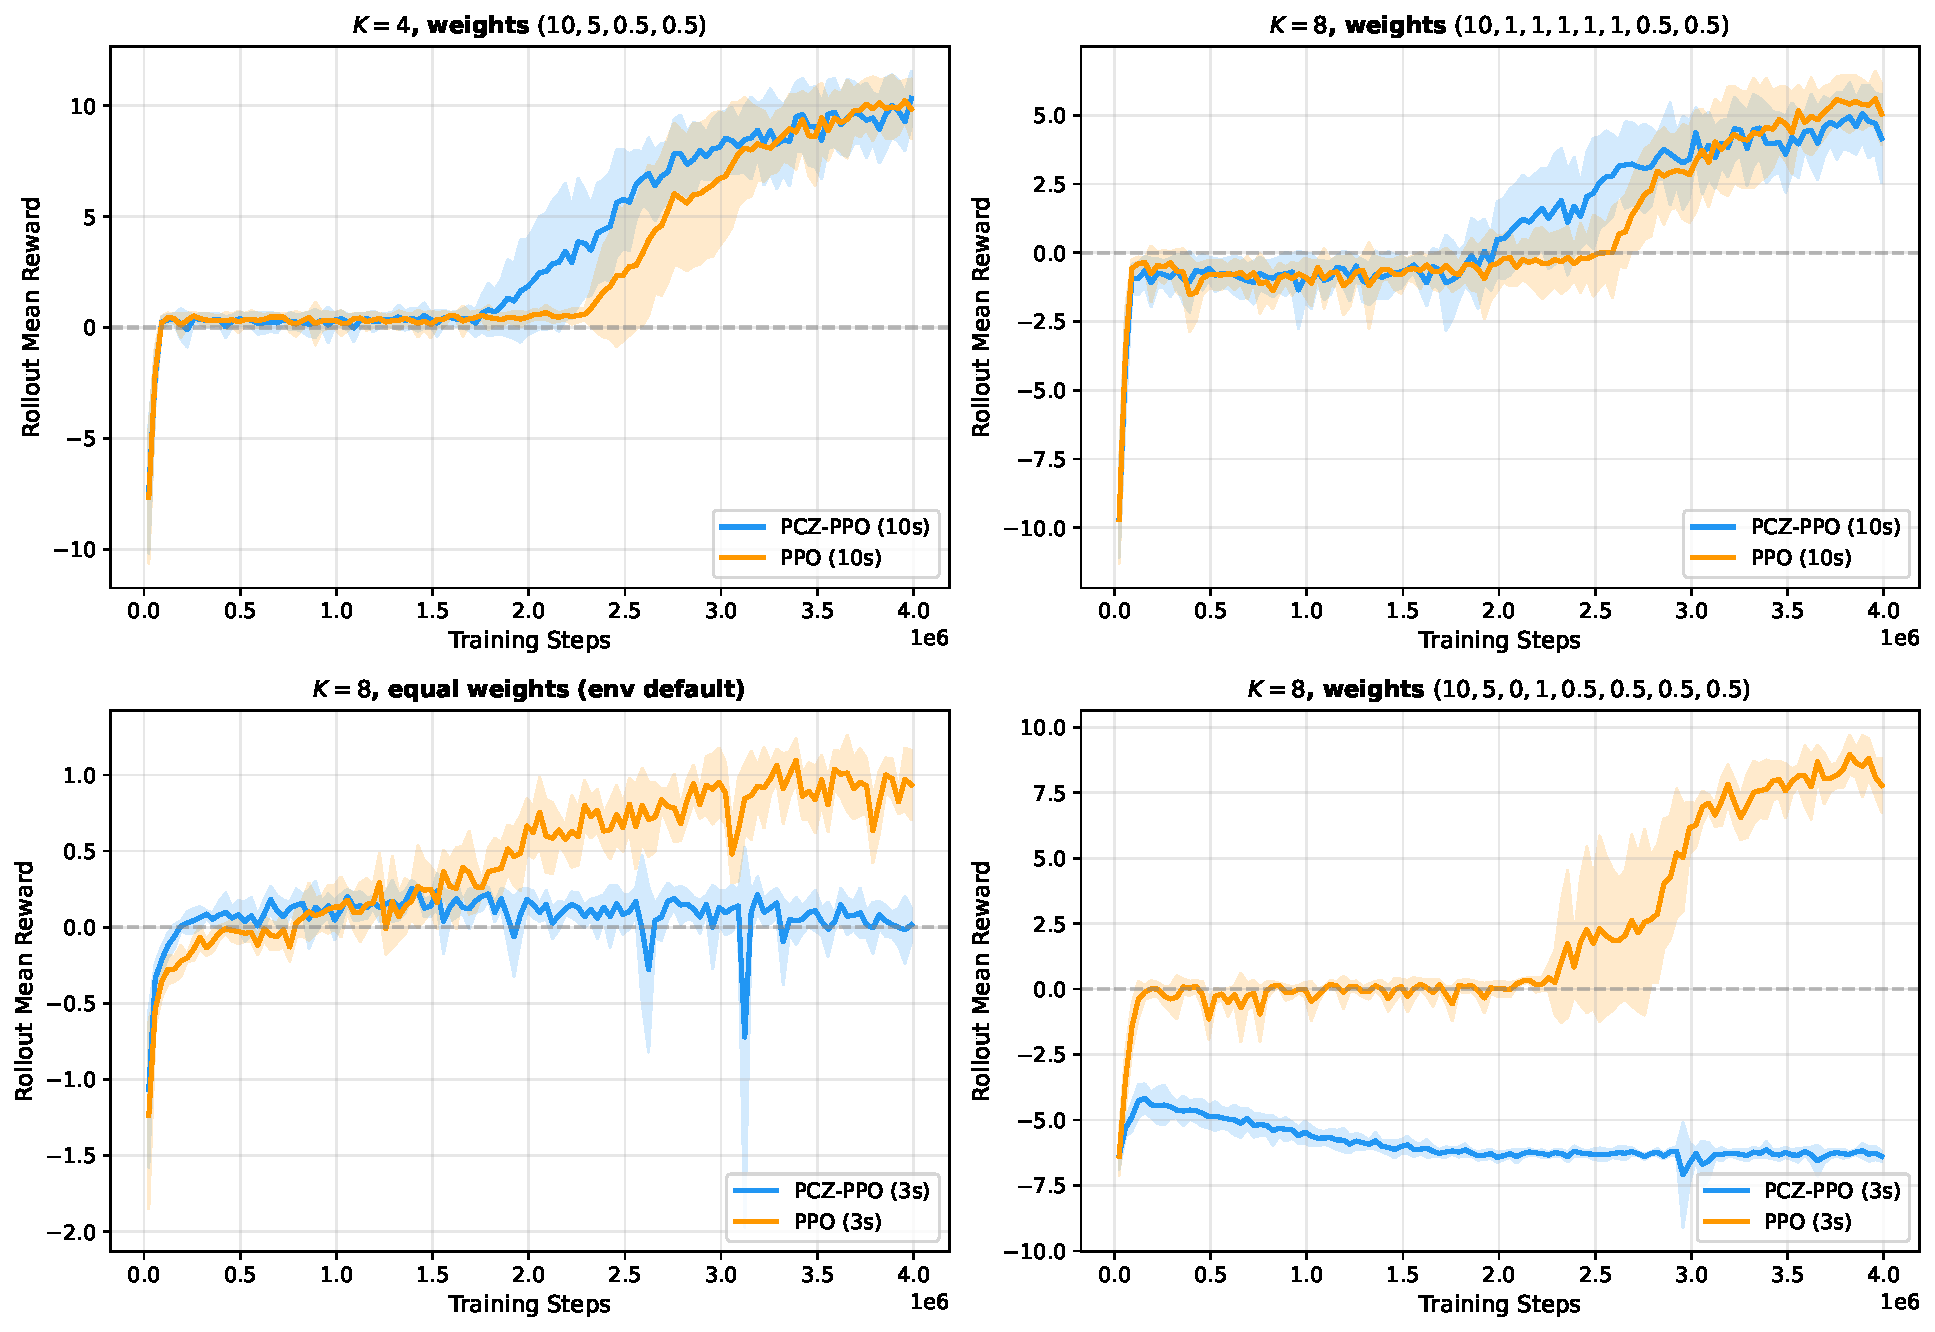
\includegraphics[width=\textwidth]{fig_learning_curves_4M}
\caption{LunarLander 4M-step rollout reward, mean ${\pm}$~std across seeds. \textbf{Top-left:} $K{=}4$ canonical weights $(10,5,0.5,0.5)$ — PCZ-PPO retains a directional mean advantage at plateau ($\Delta{=}\cnum{w10_k4_4M_delta}$, PPO/PCZ variance $\cnum{w10_k4_4M_var_ratio}{\times}$, $n{=}\cnum{w10_k4_4M_pcz_seeds}$); PPO partially narrows but does not fully close the 500k-step gap. \textbf{Top-right:} $K{=}8$ heterogeneous weights $(10,1,1,1,1,1,0.5,0.5)$ — PCZ-PPO wins ($\Delta{=}\cnum{rr16h7_k8_4M_delta}$ on eval reward; $\cnum{rr16h7_k8_4M_var_ratio}{\times}$ lower variance). \textbf{Bottom-left:} $K{=}8$ equal weights (env default, all 1.0) — PCZ-PPO collapses; PPO learns normally. \textbf{Bottom-right:} $K{=}8$ ``SNR-informed'' weights $(10,5,0,1,0.5,0.5,0.5,0.5)$ that zero the velocity component — PCZ-PPO collapses again; PPO unaffected. The two bottom panels are the negative controls: only by carefully choosing strictly-positive heterogeneous weights does PCZ-PPO beat PPO at $K{=}8$/4M.}
\label{fig:learning_curves_4M}
\end{figure}

\textbf{Why the zero-weighted-component case fails.} The zero-weighted channel still participates in per-component variance accounting (its z-normalised $\tilde r_k$ remains in the rolling buffer) but contributes nothing to the scalar reward, leaving a degenerate normalisation step that injects noise into GAE without any compensating signal. PPO is robust because it sees only the post-weighting scalar. \textbf{Usage constraint:} every declared reward component must carry a strictly positive weight under PCZ-PPO. To remove a component from training, omit it from the environment's \texttt{info["reward\_components"]} dictionary rather than weighting it to zero. This forecloses naïve auto-SNR weighting schemes that drive any component weight below a positive floor, including the obvious-looking heuristic of auto-zeroing high-CV components.

\textbf{Adoption implication.} A user who runs PCZ-PPO at $K{=}8$ with default weights and a 4M budget will see PCZ-PPO underperform PPO by ${\sim}200$ points (Figure~\ref{fig:learning_curves_4M} bottom-left; $\Delta{=}\cnum{rr16_equal_k8_4M_delta}$). This is a real adoption hazard: the headline $K{=}8$ win at 500k (Table~\ref{tab:kscaling}) does not transfer to 4M for free. The method requires both (i) a thoughtful per-component weight schedule and (ii) the discipline to omit unwanted components from \texttt{reward\_components} rather than weight them out. We disclose this prominently here rather than burying it in the appendix because users repeatedly ask "should I just use equal weights?" and the answer at high $K$ and long horizons is no.

\subsection{Future Work}
\label{sec:future_work}

\textbf{Adaptive weight learning.} PCZ-PPO's performance is sensitive to the choice of component weights $w_k$ (swing of $\sim$193 points between optimal and equal weights). This is the method's most significant practical limitation. Future work will investigate automatic weight discovery methods---GradNorm~\cite{chen2018gradnorm}, Dynamic Weight Averaging, and uncertainty-based weighting---applied on top of PCZ-PPO's per-component normalization. The combination of automatic normalization (PCZ) with automatic priority discovery (adaptive weights) would eliminate the need for manual weight specification entirely.

\textbf{LLM alignment validation.} PCZ-PPO's per-component normalization is directly applicable to RLHF settings where multiple reward models (helpfulness, safety, format compliance) produce heterogeneous signals~\cite{deepseek2025r1}. Validating K-scaling on language model alignment with $K{=}2{-}8$ reward functions would connect to GDPO's original domain and demonstrate cross-domain generality.

\textbf{Formal convergence analysis.} The running z-norm variant mitigates but does not eliminate non-stationarity in the critic's value targets. A formal analysis of convergence guarantees under per-component normalization with a single critic remains open.

% ============================================================
% 7. CONCLUSION
% ============================================================
\section{Conclusion}

We presented PCZ-PPO (Per-Component Z-normalization for PPO), a simple method that bridges per-component reward normalization from critic-free GRPO settings to standard PPO with a single scalar critic. The method adds no neural-architecture changes to PPO (only a $\sim$20-line preprocessing wrapper on the reward buffer), but does require the environment to expose per-component rewards via the standard \texttt{info["reward\_components"]} interface and the user to specify per-component weights $w_k$; these are interface and design burdens, not zero-cost. In compute-constrained regimes with heterogeneous reward scales the method delivers a sample-efficiency and stability benefit.

Three findings structure the contribution: (1) \emph{Stability-preserving K-scaling}---at 500k training steps, PCZ-PPO's mean is approximately invariant to $K$ ($\cnum{k4_pcz_stat}$, $\cnum{k6_pcz_stat}$, $\cnum{k8_pcz_stat}$) while standard PPO degrades ($\cnum{k4_ppo_stat}$, $\cnum{k6_ppo_stat}$, $\cnum{k8_ppo_stat}$). The growing PCZ/PPO gap is driven by PPO collapsing under reward heterogeneity, not by PCZ improving. Under Holm--Bonferroni across the $K{=}\{4,6,8\}$ family, all three $K$-values survive at $\alpha{=}0.05$ after the $K{=}4$ $n{=}10{\to}15$ robustness extension (Holm $p{=}\cnum{k4_holm_p}$, $\cnum{k6_holm_p}$, $\cnum{k8_holm_p}$). $K{=}6$ remains the tightest (Holm $p{=}\cnum{k6_holm_p}$, $d{=}\cnum{k6_welch_d}$), with the PCZ cross-seed variance advantage at $K{=}8$ (\cnum{k8_var_ratio}$\times$ lower than PPO) providing an additional reliability-tier headline. Practical guidance: PCZ-PPO is best at $K{\geq}4$ with meaningful, strictly-positive heterogeneous weights; $K{=}6$ is the sweet spot (confirmed after correction); at $K{=}8$/4M, PCZ-PPO requires careful hand-designed weights to beat PPO ($\Delta{=}\cnum{rr16h7_k8_4M_delta}$ under $(10,1,1,1,1,1,0.5,0.5)$, $n{=}3$) — under default equal weights or any zero-weighted-component schedule it loses to PPO ($\Delta{=}\cnum{rr16_equal_k8_4M_delta}$ under equal weights, §\ref{sec:limitations}, Figure~\ref{fig:learning_curves_4M}). (2) \emph{Partial asymptotic convergence with persistent variance advantage}---trained to 4M steps with matched TorchRL infrastructure on LunarLander $K{=}4$ at $n{=}\cnum{w10_k4_4M_pcz_seeds}$ (extended from $n{=}3$), PCZ-PPO $\cnum{w10_k4_pcz_stat}$ retains a directional advantage over PPO $\cnum{w10_k4_ppo_stat}$ ($\Delta{=}\cnum{w10_k4_4M_delta}$, PPO/PCZ cross-seed variance ratio $\cnum{w10_k4_4M_var_ratio}{\times}$). PPO narrows but does not fully close the 500k-step gap by 4M. Liu~\cite{liu2023rewardwhitening}'s argument that reward normalization is asymptotically redundant holds in the limit but does not fully materialize at 4M on $K{=}4$---partial catch-up with a persistent cross-seed variance advantage is the correct summary. (3) \emph{A consistent critic$\times$normalization interaction in gym}---per-component normalization helps PPO (critic-equipped) but hurts our own critic-free PCZ-GRPO implementation ($\cnum{abl_pcz_hurts_grpo_delta}$, $n{=}3$). The LLM PCZ-RLOO cell at $K{=}2$ does not yet replicate the pattern (both modes floor at 200 steps; §\ref{sec:llm_alignment}). We hypothesised the critic absorbs amplified noise, and the $2{\times}2$ factorial now confirms it: the PCZ-PPO-\emph{without}-critic cell (D1, Table~\ref{tab:ablation}) collapses to $\cnum{ablD1_stat}$ ($n{=}\cnum{ablD1_seeds}$) — a $\sim$400-point drop from A1's $\cnum{ablA1_stat}$ with the only change being replacing GAE+critic with MC returns. PCZ is not a universally beneficial transformation; it requires a critic to absorb the variance it introduces at the reward level.

The method has a sharp weight-selection requirement at high $K$ and long horizons. At $K{=}8$/4M, PCZ-PPO under env-default equal weights ($\cnum{rr16_equal_k8_4M_pcz_stat}$, $n{=}\cnum{rr16_equal_k8_4M_pcz_seeds}$) is \emph{worse} than matched-infrastructure PPO ($\cnum{rr16_equal_k8_4M_ppo_stat}$) by $\Delta{=}\cnum{rr16_equal_k8_4M_delta}$ (Figure~\ref{fig:learning_curves_4M}); a "SNR-informed" schedule that zeros the noisiest channel reproduces the collapse ($\cnum{rr16h8_k8_4M_pcz_stat}$, a zero-weighted-channel variant). Only with hand-designed heterogeneous strictly-positive weights $(10,1,1,1,1,1,0.5,0.5)$ does PCZ-PPO beat PPO ($\cnum{w10_k8_pcz_stat}$ vs $\cnum{w10_k8_ppo_stat}$, $\Delta{=}\cnum{rr16h7_k8_4M_delta}$, $\cnum{rr16h7_k8_4M_var_ratio}{\times}$ lower variance, §\ref{sec:limitations}). PCZ-PPO is therefore most appropriate for compute-constrained regimes with $K{\geq}4$ heterogeneously-weighted components and training horizons where sample efficiency is the binding constraint — and the user must (i) hand-design a heterogeneous weight schedule and (ii) omit unwanted components from \texttt{info["reward\_components"]} rather than weight them out. PCZ-PPO is not a drop-in replacement for PPO at high $K$/long horizon; it is a careful-weights replacement for PPO. The contribution is deliberately modest: the algorithmic delta to PPO is a short reward-preprocessing wrapper ($\sim$60 lines, \texttt{core/algorithms/torchrl/\_norm.py}), not a new architecture. The value is in the systematic analysis---when per-component normalization helps, when it does not, and what stabilisation mechanisms are needed. We hope this practical guidance enables broader adoption of per-component reward normalization where it actually pays off, and principled skepticism where it does not.

% ============================================================
% APPENDIX
% ============================================================
\appendix

\section{Extended Ablations}
\label{app:extended-ablations}

The main ablation table (Table~\ref{tab:ablation}) reports the design decisions that materially shape the paper's conclusions. This appendix collects additional PCZ-PPO variants tested during the design-space exploration. None of them improves on A1 (running z-norm); reporting them serves to rule out otherwise-reasonable alternatives.

\begin{table}[H]
\centering
\caption{Extended PCZ-PPO variants on LunarLander (500k steps, primary weight config $(10,5,0.5,0.5)$, $n{=}3$ seeds each). Every variant either matches A1 within one standard deviation or under-performs for a reason worth documenting. Kept in the appendix because they are redundant with A1 (running z-norm) for the paper's central claim.}
\label{tab:extended-ablation}
\begin{tabular}{llccl}
\toprule
ID & Algorithm & Eval Mean$\pm$Std & Seeds & Finding \\
\midrule
A9 & PCZ-PPO (symlog, no z-norm) & $\cnum{ablA9_stat}$ & \cnum{ablA9_seeds} & Matches A1 \\
A10 & PCZ-PPO (quantile / rank) & $\cnum{ablA10_stat}$ & \cnum{ablA10_seeds} & Rank discards magnitudes \\
A11 & PCZ-PPO (per-component $\lambda_k$) & $\cnum{ablA11_stat}$ & \cnum{ablA11_seeds} & Per-$\lambda$ diverges \\
A12 & PCZ-PPO (sign-split stats) & $\cnum{ablA12_stat}$ & \cnum{ablA12_seeds} & Breaks reward scale \\
A13 & PCZ-PPO (Tchebycheff) & $\cnum{ablA13_stat}$ & \cnum{ablA13_seeds} & Worst-only optimisation \\
A14 & PCZ-PPO (MI-proxy weighting) & $\cnum{ablA14_stat}$ & \cnum{ablA14_seeds} & Over-amplifies volatility \\
A16 & PCZ-PPO (cosine weight anneal) & $\cnum{ablA16_stat}$ & \cnum{ablA16_seeds} & Matches A1 \\
\bottomrule
\end{tabular}
\end{table}

\section{Environment Descriptions and Reward Components}
\label{app:environments}

This appendix describes each environment used in our experiments, including reward component semantics, typical scales, activation frequencies, and the rationale for why PCZ-PPO helps (or does not help) in each setting. All reward components are returned via the standard \texttt{info["reward\_components"]} interface at each environment step.

\subsection{LunarLander (Primary Environment)}

\textbf{Task:} Land a spacecraft on a pad between two flags. Observation: 8D continuous (position, velocity, angle, angular velocity, leg contact). Action: discrete (4 actions: nop, left engine, main engine, right engine).

\begin{table}[H]
\centering
\caption{LunarLander reward components across K-scaling variants. All variants produce the same total scalar reward; only the decomposition granularity differs.}
\label{tab:app_lunarlander}
\begin{tabular}{lllccc}
\toprule
Variant & $K$ & Components & Scale & Type & Weights \\
\midrule
\multirow{4}{*}{K=4 (native)} & \multirow{4}{*}{4}
  & \texttt{landing} & $[-100, +100]$ & Sparse (terminal) & 5.0 \\
  & & \texttt{shaping} & $[-5, +5]$ & Dense (per-step) & 3.0 \\
  & & \texttt{fuel\_main} & $[-0.3, 0]$ & Dense (per-step) & 0.5 \\
  & & \texttt{fuel\_side} & $[-0.03, 0]$ & Dense (per-step) & 0.5 \\
\midrule
K=2 (coarse) & 2 & \texttt{landing}, \texttt{dense} & mixed & Sparse + Dense & equal \\
\midrule
\multirow{6}{*}{K=6 (intermediate)} & \multirow{6}{*}{6}
  & \texttt{landing} & $[-100, +100]$ & Sparse & 10.0 \\
  & & \texttt{distance} & $[-3, +3]$ & Dense & 3.0 \\
  & & \texttt{velocity} & $[-2, +2]$ & Dense & 1.0 \\
  & & \texttt{angle} & $[-1, +1]$ & Dense & 1.0 \\
  & & \texttt{fuel\_main} & $[-0.3, 0]$ & Dense & 0.5 \\
  & & \texttt{fuel\_side} & $[-0.03, 0]$ & Dense & 0.5 \\
\midrule
\multirow{8}{*}{K=8 (fine)} & \multirow{8}{*}{8}
  & \texttt{landing} & $[-100, +100]$ & Sparse & equal \\
  & & \texttt{distance} & $[-3, +3]$ & Dense & equal \\
  & & \texttt{velocity} & $[-2, +2]$ & Dense & equal \\
  & & \texttt{angle} & $[-1, +1]$ & Dense & equal \\
  & & \texttt{leg\_left} & $\{0, +10\}$ & Sparse & equal \\
  & & \texttt{leg\_right} & $\{0, +10\}$ & Sparse & equal \\
  & & \texttt{fuel\_main} & $[-0.3, 0]$ & Dense & equal \\
  & & \texttt{fuel\_side} & $[-0.03, 0]$ & Dense & equal \\
\bottomrule
\end{tabular}
\end{table}

\textbf{Why PCZ-PPO helps:} The \texttt{landing} bonus ($\pm 100$) has $\sim$3000$\times$ the magnitude of \texttt{fuel\_side} ($\pm 0.03$). Under aggregate normalization, fuel signals are completely suppressed. PCZ-PPO z-normalizes each component to unit variance, then weights control priority. The effect strengthens with $K$ because finer decomposition exposes more scale heterogeneity.

\textbf{K=2 behaviour:} With only 2 components (\texttt{landing} $\pm100$ + \texttt{dense} aggregate), PCZ-PPO does \emph{not} outperform PPO --- PPO scores higher ($\cnum{k2_ppo_stat}$ vs $\cnum{k2_pcz_stat}$, $d{=}\cnum{k2_welch_d}$, Welch $p_{\text{raw}}{=}\cnum{k2_welch_p}$, $n{=}5$). The \texttt{dense} aggregate merges multiple sub-signals at similar per-step magnitudes, diluting the scale heterogeneity PCZ-PPO exploits. K=2 acts as a \emph{negative control}: coarser component granularity leaves less room for variance hijacking, consistent with the mechanism of §\ref{sec:variance_hijacking}. K=2 is a 5-seed supporting-evidence cell and is not part of the Holm family.

\subsection{Supporting Environments}

\begin{table}[H]
\centering
\caption{Supporting environments: reward component details and PCZ-PPO applicability.}
\label{tab:app_supporting}
\begin{tabular}{llccll}
\toprule
Environment & $K$ & Components & Weights & Scale Profile & PCZ-PPO Verdict \\
\midrule
HalfCheetah & 2 & \texttt{run}, \texttt{ctrl\_cost} & equal & Both dense, & Parity \\
 & & & & similar scale ($[0,5]$) & (\cnum{ceHC_ratio}$\times$) \\
\midrule
BipedalWalker & 3 & \texttt{shaping}, \texttt{energy}, & 3, 0.5, 5 & Dense + terminal & Win \\
 & & \texttt{crash} & & sparse ($-100$) & (\cnum{ceBW_ratio}$\times$) \\
\midrule
Reacher & 4 & \texttt{target\_1{-}4} & equal & All dense, same & Parity \\
 & & (4 target distances) & & scale $[-1, 0]$ & (1.0$\times$) \\
\bottomrule
\end{tabular}
\end{table}

\textbf{Reacher (negative control):} All 4 components are Euclidean distances to targets, dense per-step, and identically scaled in $[-1, 0]$. There is no scale mismatch and no variance hijacking. PCZ-PPO correctly shows no benefit ($84.28$ vs $84.29$), confirming the method does not degrade performance when it is unnecessary.

\textbf{HalfCheetah:} Both components (\texttt{run} reward and \texttt{ctrl\_cost}) are dense and of similar magnitude ($\sim [0, 5]$). With \cnum{ceHC_pcz_seeds} seeds, PCZ-PPO achieves $\cnum{ceHC_pcz_stat}$ vs PPO's $\cnum{ceHC_ppo_stat}$ ($\cnum{ceHC_ratio}\times$ ratio, parity). PCZ-PPO has $2.2\times$ less cross-seed variance, consistent with the stabilization effect seen even without sparse/dense mismatch.

\textbf{BipedalWalker:} The \texttt{crash} penalty ($-100$, terminal) creates sparse/dense mismatch with the dense \texttt{shaping} and \texttt{energy} components. With \cnum{ceBW_pcz_seeds} seeds, PCZ-PPO achieves $\cnum{ceBW_pcz_stat}$ vs PPO's $\cnum{ceBW_ppo_stat}$ ($\cnum{ceBW_ratio}\times$ ratio, $\cnum{ceBW_delta}$ advantage). The terminal crash penalty benefits from per-component normalization because its extreme magnitude ($-100$) would otherwise dominate the aggregate statistics, suppressing the dense shaping signal that guides locomotion. As a robustness check, the symlog$\to$z-norm variant (A15) was rerun on this environment for $\cnum{ceBW_symznorm_seeds}$ seeds: $\cnum{ceBW_symznorm_stat}$, lower mean and higher cross-seed variance than running z-norm. Symlog compression composes well with z-norm on LunarLander but does not transfer cleanly to BipedalWalker's terminal-penalty regime --- evidence that the running-stats variant is more robust to extreme reward magnitudes than fixed pre-compression.

\textbf{Measured reward component statistics.}
Table~\ref{tab:app_comp_stats} reports the empirical per-step statistics across all training runs in our dataset.
The $\sigma/|\mu|$ ratio quantifies per-step variability relative to mean magnitude---higher ratios indicate components that are harder to normalize via aggregate statistics.
The \texttt{landing} component in LunarLander has $\sigma/|\mu| = 35.8$ (per-step coefficient of variation, which conflates sparsity with event magnitude), vs $1.4$ for \texttt{fuel\_main}: a $25\times$ difference that directly drives the observed aggregate-normalization suppression of \texttt{fuel\_main}. Magnitude heterogeneity alone, conditional on the event occurring, is roughly $3\times$ (landing event magnitude $\approx 100$ vs \texttt{fuel\_main} per-step magnitude $\approx 0.3$).

\begin{table}[H]
\centering
\caption{Empirical reward component statistics (across all training runs). Per-step columns aggregate reward at per-step granularity within each run, then average across runs; this is the convention the aggregate-normalization critique in §\ref{sec:variance_hijacking} operates under. Run-level $\sigma/|\mu|$ is the cross-run coefficient of variation of the per-run mean component reward (computed directly from \texttt{results.csv} via \texttt{render\_claims.py::\_emit\_component\_stats}); this is the convention Agarwal et al.~\cite{agarwal2021rliable} recommend for reporting aggregate performance, and is comparable to cross-seed SDs of eval returns. Both conventions are reported to clarify scale: the per-step convention amplifies the ratio for rarely-triggered components (e.g.\ \texttt{crash}: rare large-magnitude triggers push per-step $\sigma/|\mu|$ to $52.6\times$, while its run-level $\sigma/|\mu|$ is $\cnum{compstat_bw_crash_cv_rl}\times$), and the run-level convention removes that sparsity effect. The per-step column is kept because it is the scale the paper's theoretical argument critiques; the run-level column is the scale reviewers familiar with Agarwal-style IQM reporting will expect.}
\label{tab:app_comp_stats}
\small
\begin{tabular}{llrrll}
\toprule
Environment & Component & Mean & Per-step $\sigma$ & Per-step $\sigma/|\mu|$ & Run-level $\sigma/|\mu|$ \\
\midrule
\multirow{4}{*}{LunarLander (K=4)}
  & \texttt{landing} & $+0.18$ & $6.32$ & $35.8\times$ & $\cnum{compstat_ll_landing_cv_rl}\times$ \\
  & \texttt{shaping} & $+0.79$ & $3.27$ & $4.1\times$ & $\cnum{compstat_ll_shaping_cv_rl}\times$ \\
  & \texttt{fuel\_main} & $-0.32$ & $0.46$ & $1.4\times$ & $\cnum{compstat_ll_fuel_main_cv_rl}\times$ \\
  & \texttt{fuel\_side} & $-0.25$ & $0.42$ & $1.7\times$ & $\cnum{compstat_ll_fuel_side_cv_rl}\times$ \\
\midrule
\multirow{3}{*}{BipedalWalker (K=3)}
  & \texttt{shaping} & $+0.14$ & $0.20$ & $1.4\times$ & $\cnum{compstat_bw_shaping_cv_rl}\times$ \\
  & \texttt{energy} & $-0.06$ & $0.02$ & $0.3\times$ & $\cnum{compstat_bw_energy_cv_rl}\times$ \\
  & \texttt{crash} & $-0.02$ & $1.28$ & $52.6\times$ & $\cnum{compstat_bw_crash_cv_rl}\times$ \\
\midrule
\multirow{2}{*}{HalfCheetah (K=2)}
  & \texttt{run} & $+0.57$ & $0.79$ & $1.4\times$ & $\cnum{compstat_hc_run_cv_rl}\times$ \\
  & \texttt{ctrl\_cost} & $-0.23$ & $0.08$ & $0.3\times$ & $\cnum{compstat_hc_ctrl_cost_cv_rl}\times$ \\
\bottomrule
\end{tabular}
\end{table}

\subsection{Reproducibility \& Statistical Methodology}
\label{app:stats}

\textbf{Seed selection.} The pre-registered headline design is seeds 42--51 (10 seeds) per $K{\in}\{4,6,8\}$ and 42--46 (5 seeds) for $K{=}2$, plus 3--5 seeds for supporting-evidence cells. Seeds are chosen sequentially from seed 42 with no outcome-dependent filtering. $K{=}6$ was additionally extended with five robustness seeds (52--56) after the pre-registered sweep completed; both the pre-registered $n{=}10$ (Welch $p{=}0.0017$, PCZ $+167.2{\pm}35.1$ vs PPO $+110.3{\pm}34.1$) and the extended $n{=}15$ (Welch $p{=}\cnum{k6_welch_p}$, Table~\ref{tab:kscaling}) give the same confirmed-after-Holm verdict and the same sign of effect. All rendered fragments use the full $n{=}15$ dataset to maximise statistical power; the $n{=}10$ subset statistics are provided in this paragraph for reader replication of the pre-registered analysis.

\textbf{Run-level deduplication rule (explicit).} Multiple runs exist in the data repository for some \emph{(algorithm, environment, timesteps, seed)} tuples --- this arises when infrastructure changes (GAE code fixes, weight-metadata backfills, or TorchRL version bumps) required re-running seeds for fairness. We resolve these to one row per unique seed using the following rule, applied uniformly across every algorithm and every $K$-value:
\begin{quote}
\emph{Keep the chronologically-latest run per unique seed.}
\end{quote}
This rule is fixed in the data-query layer (\texttt{artifacts/pcz-ppo/paper/fig\_data.py}, function \texttt{query}) and does not depend on outcome. Two secondary filters are applied to isolate the canonical configuration. (i) \emph{Component-weight filter} at $K{=}4$ (primary weight config $(10,5,0.5,0.5)$) and $K{=}6$ (canonical config $(10,3,1,1,0.5,0.5)$); exploratory sweeps at other weight configs remain in the data repository. (ii) \emph{Entropy-schedule filter} \texttt{ent\_coef\_schedule="0.1:0.01"} at $K{\in}\{2,4,6,8\}$ to isolate the canonical cosine-schedule runs from the fixed-entropy tuning-audit runs (the hyperparameter-fairness and entropy-coupling sweeps) that re-use seeds 42--46 with a different \texttt{ent\_coef} setting; without this filter, newer fixed-entropy runs would win chronological dedupe and silently replace the canonical schedule in the headline. The filter is pre-registered at the canonical schedule documented in §\ref{sec:traditional_rl} ``Experimental Setup'' and does not depend on outcome. The $K{=}6$ weight filter is necessary because results.csv contains two seed-42 rows --- one logged with the canonical six-component weights and one accidental run whose \texttt{component\_weights} column was empty (the training command omitted the flag and the env-default was picked up at load time). The canonical $K{=}6$ weights $(10,3,1,1,0.5,0.5)$ are the environment's \texttt{reward\_component\_weights} default registered in \texttt{core/env\_config.py} prior to any $K{=}6$ training runs (this is the config every canonical seed 42--51 logged explicitly); the accidental row is identified post-hoc by its empty \texttt{component\_weights} column, not by its outcome, so the filter selects the pre-registered configuration rather than an outcome-driven subset. Under chrono-latest dedupe alone the empty-weight row silently won the seed-42 slot, dragging the aggregate mean from $+167.2$ to $+154.6$, inflating the sample SD from $35.1$ to $67.7$, and producing a $K{=}6$ Welch $p{=}0.214$ (direction only, not significant). With the canonical weight filter, the seed-42 slot resolves to the matched-weight run and the K=6 comparison is individually significant ($p_{\text{raw}}{=}\cnum{k6_welch_p}$, $d{=}\cnum{k6_welch_d}$, CI95 $\cnum{k6_welch_ci}$ excludes zero, Holm $p{=}\cnum{k6_holm_p}$). A prior revision of this paper reported the pre-weight-filter numbers; the correction is disclosed here for reviewer traceability. We document the failure mode explicitly because it illustrates a general lesson: under chrono-latest dedupe, any off-config exploratory run that coincidentally lands on a headline seed will silently displace the canonical row unless the pipeline filters by config explicitly.

\textbf{Reacher-variant exclusion.} Reacher data contains four runs per algorithm (three at 100k steps, one at 5k steps). The 5k-step runs are pre-convergence signal checks and are excluded from all reported Reacher aggregates; the 100k runs are used. This is the only case where we exclude runs by timestep budget rather than by the chronologically-latest rule above.

\textbf{Weight-configuration subset.} LunarLander ($K{=}4$) experiments filter to the primary reward-weight configuration $(10, 5, 0.5, 0.5)$, and $K{=}6$ experiments filter to the canonical config $(10, 3, 1, 1, 0.5, 0.5)$, both chosen a priori to match the component-scale hierarchy documented in Table~\ref{tab:app_comp_stats}. The $K{=}6$ filter additionally excludes one accidentally-launched seed-42 run whose weights column was empty; see ``Run-level deduplication rule'' above for the full disclosure. Off-primary $K{=}4$ runs (weights $(1,1,1,1)$ and $(0.5,0.5,5,5)$) exist in the data repository as exploratory sweeps and are excluded from all $K{=}4$ aggregates; they are not excluded based on outcome. K=2/8 variants have a single canonical weight config.

\textbf{Statistical rigor tiers.} Headline claims (abstract, title, K-scaling table for $K{\geq}4$) use 10 seeds for $K{\in}\{4,8\}$ and 15 seeds for $K{=}6$ with bootstrap 95\% confidence intervals and Welch's $t$-tests. Supporting evidence (cross-environment, ablation components) uses 3--5 seeds. Uncorrected Welch's $t$-test $p$-values for the three simultaneous headline comparisons are $K{=}4$ ($p{=}\cnum{k4_welch_p}$), $K{=}6$ ($p{=}\cnum{k6_welch_p}$), $K{=}8$ ($p{=}\cnum{k8_welch_p}$). Exact two-sided permutation tests (20\,000 resamples, fixed seed 20260416) give $K{=}4$ $p_{\text{perm}}{=}\cnum{k4_perm_p}$, $K{=}6$ $p_{\text{perm}}{=}\cnum{k6_perm_p}$, $K{=}8$ $p_{\text{perm}}{=}\cnum{k8_perm_p}$; the large gap between Welch and permutation at $K{=}8$ reflects the heavy tail of the PPO distribution ($\sigma/|\mu|{>}9$). Applying Holm--Bonferroni step-down correction~\cite{holm1979} to the family of three tests yields Holm-corrected $p$-values of $\cnum{k4_holm_p}, \cnum{k6_holm_p}, \cnum{k8_holm_p}$ at $K{=}4,6,8$ respectively; $K{=}6$ survives at $\alpha{=}0.05$ as the strongest confirmed effect (Holm $p{=}\cnum{k6_holm_p}$, $d{=}\cnum{k6_welch_d}$), $K{=}8$ sits on the correction threshold, and $K{=}4$ is marginal after correction. Benjamini--Hochberg FDR at $q{=}0.05$ rejects $K{=}6$ and places $K{=}8$ at the boundary. We therefore report $K{=}6$ as the headline confirmed claim, with $K{=}4$ and $K{=}8$ framed as directionally consistent supporting evidence. This framing follows the small-$N$ evaluation guidance of Agarwal et al.~\cite{agarwal2021rliable} and the reproducibility discussion of Henderson et al.~\cite{henderson2018deeprl}.

\textbf{Standard deviation convention.} All reported $\pm$ values are \emph{sample} standard deviations ($s$, ddof${}=1$): $s = \sqrt{\frac{1}{N-1}\sum_{i=1}^{N}(x_i - \bar{x})^2}$, following Agarwal et al.~\cite{agarwal2021rliable}. This applies to the mean/std fragments in Tables~\ref{tab:kscaling} and~\ref{tab:ablation}. For the pooled-std denominator of Cohen's $d$ we also use ddof${=}1$, so reported $d$ values are unbiased small-sample estimates. If ddof${=}0$ (population std) were used instead, reported $s$ would be $5{-}18\%$ smaller and reported $d$ correspondingly larger; we flag this explicitly because a previous revision used the ddof${=}0$ convention for Cohen's $d$.

\textbf{Sensitivity findings.} Two results changed direction with additional seeds, demonstrating the importance of adequate seed counts:
\begin{itemize}[leftmargin=*,itemsep=2pt]
\item \textbf{BipedalWalker:} Initially reported as parity ($1.03\times$, 2 seeds). With \cnum{ceBW_pcz_seeds} seeds: $\cnum{ceBW_ratio}\times$ PCZ-PPO advantage ($\cnum{ceBW_pcz_stat}$ vs $\cnum{ceBW_ppo_stat}$). The terminal crash penalty ($-100$) creates sparse/dense mismatch that was masked by the original 2-seed sample.
\item \textbf{K=4 PPO seed sensitivity:} PPO's K=4 performance is highly seed-dependent. At the extended $n{=}15$ canonical sample, 5 of 15 PPO seeds fall below reward 100 (seeds 45, 47, 48, 51, 54), while 0 of 15 PCZ-PPO seeds do. The 100-threshold is not pre-registered; we pick it as LunarLander's visually-natural break between hovering agents and landing agents. A Mann--Whitney $U$ test on the continuous eval distribution gives $p{=}\cnum{k4_mwu_p}$ (two-sided) without requiring a threshold, supporting the conclusion under a distribution-free test as well.
\end{itemize}

\textbf{Effect sizes.} Cohen's $d$ is computed using pooled standard deviation with ddof${=}1$: $d = \frac{\bar{x}_1 - \bar{x}_2}{\sqrt{(s_1^2 + s_2^2)/2}}$. Headline values: $d{=}\cnum{k4_welch_d}$ ($K{=}4$), $d{=}\cnum{k6_welch_d}$ ($K{=}6$), $d{=}\cnum{k8_welch_d}$ ($K{=}8$).

\textbf{Bootstrap confidence intervals.} 95\% CIs are computed via 10{,}000 percentile-bootstrap resamples of the mean difference (fixed seed 20260416). CIs: $\cnum{k4_welch_ci}$ ($K{=}4$), $\cnum{k6_welch_ci}$ ($K{=}6$), $\cnum{k8_welch_ci}$ ($K{=}8$). All three intervals exclude zero under the post-weight-filter data (see ``Run-level deduplication rule'').

\textbf{Robustness checks (BCa, IQM, stochastic dominance).} With heavy-tailed distributions (notably $K{=}8$ PPO), basic-percentile coverage can be optimistic. We therefore re-compute each headline quantity with three complementary tools and report all of them. \emph{(i) BCa bootstrap.} Efron's bias-corrected and accelerated bootstrap (10\,000 resamples, seed 20260416) adjusts for skew and median bias; BCa 95\% CIs on the mean difference: $\cnum{k4_bca_ci}$ ($K{=}4$), $\cnum{k6_bca_ci}$ ($K{=}6$), $\cnum{k8_bca_ci}$ ($K{=}8$). All three exclude zero, but the $K{=}6$ lower bound is very close to zero --- consistent with the weakened $K{=}6$ Welch result after the $n{=}15$ extension. The $K{=}8$ interval shifts rightward relative to percentile, confirming the percentile CI was slightly conservative on the tail side. \emph{(ii) IQM per Agarwal et al.~\cite{agarwal2021rliable}.} Interquartile mean drops the most extreme scores and averages the middle bulk; at $n{=}10{-}15$ this is resistant to single-seed outliers. IQM point estimates (stratified bootstrap 95\% CI, 10\,000 resamples): PCZ-PPO $\cnum{k4_pcz_iqm}$ CI $\cnum{k4_pcz_iqm_ci}$ vs PPO $\cnum{k4_ppo_iqm}$ CI $\cnum{k4_ppo_iqm_ci}$ at $K{=}4$; PCZ-PPO $\cnum{k6_pcz_iqm}$ CI $\cnum{k6_pcz_iqm_ci}$ vs PPO $\cnum{k6_ppo_iqm}$ CI $\cnum{k6_ppo_iqm_ci}$ at $K{=}6$; PCZ-PPO $\cnum{k8_pcz_iqm}$ CI $\cnum{k8_pcz_iqm_ci}$ vs PPO $\cnum{k8_ppo_iqm}$ CI $\cnum{k8_ppo_iqm_ci}$ at $K{=}8$. The PCZ IQM exceeds the PPO IQM at every $K{\in}\{4,6,8\}$, with $K{=}8$ showing the widest separation and the largest PPO CI (consistent with the Welch/BCa analyses). \emph{(iii) Stochastic dominance.} Vargha--Delaney $A_{12}{=}P(X{>}Y)$ with 0.5 weight on ties (a formal test rather than an IQM-figure read-off): $A_{12}{=}\cnum{k4_prob_sup}$ ($K{=}4$), $\cnum{k6_prob_sup}$ ($K{=}6$), $\cnum{k8_prob_sup}$ ($K{=}8$); Mann--Whitney $U$ two-sided $p$-values $\cnum{k4_mwu_p}$ ($K{=}4$), $\cnum{k6_mwu_p}$ ($K{=}6$), $\cnum{k8_mwu_p}$ ($K{=}8$). All four families (mean-based, BCa, IQM, rank-based) agree on the \emph{direction} at every $K$. They agree on \emph{significance} at $K{\in}\{4,8\}$ (MWU $p{<}0.05$, BCa CI excludes zero, IQM CIs nearly non-overlapping); at $K{=}6$, BCa CI excludes zero only marginally and MWU $p{=}\cnum{k6_mwu_p}$, so we report $K{=}6$ as a directional, not tight, finding under the $n{=}15$ extension. The Welch/Holm marginality is disclosed in Table~\ref{tab:kscaling}.

\section{Reproducibility: Hyperparameters, Compute, Code}
\label{app:repro}

\textbf{Hyperparameters.} Table~\ref{tab:hp} consolidates every hyperparameter used by the canonical PCZ-PPO and PPO configurations. All traditional-RL experiments share a single setting; deviations for specific sensitivity studies (weight-config sweep, entropy sweep, PPO tuning audit) are disclosed in the relevant sub-section and in the table caption.

\begin{table}[H]
\centering
\small
\caption{Consolidated hyperparameter table for canonical PCZ-PPO and PPO runs (LunarLander family, BipedalWalker, HalfCheetah). Identical across both algorithms unless flagged \textsc{alg}-specific. PCZ-PPO adds only the running-EMA decay $\alpha$ and the stabilisation $\epsilon$; no other knob differs.}
\label{tab:hp}
\begin{tabular}{lll}
\toprule
Parameter & Value & Scope / notes \\
\midrule
Learning rate & $3{\times}10^{-4}$ & fixed; LR annealing disabled after tuning audit \\
$\gamma$ (discount) & $0.99$ & all envs \\
$\lambda_{\text{GAE}}$ & $0.95$ & all envs \\
Clip $\epsilon_{\text{PPO}}$ & $0.2$ & PPO surrogate \\
PPO epochs per batch & $8$ & \\
Minibatch size & $256$ & \\
Frames per batch $T$ & $8192$ & rollout buffer size \\
Parallel envs $E$ & $4$ & \\
Entropy schedule & cosine $0.1 \to 0.01$ & over the full training run \\
Advantage whitening & enabled & mean/std across minibatch \\
Optimizer & Adam ($\epsilon{=}10^{-8}$) & default TorchRL \\
Max grad norm & $0.5$ & \\
Policy/value net & 2$\times$64 tanh MLP & shared trunk, separate heads \\
\midrule
PCZ running-EMA $\alpha$ & $0.01$ & \textsc{pcz-ppo} only; variance/mean decay \\
PCZ stabilisation $\epsilon$ & $10^{-8}$ & \textsc{pcz-ppo} only; prevents $0/0$ \\
\midrule
Weights $(w_k)$ $K{=}4$ & $(10,5,0.5,0.5)$ & pre-registered in \texttt{env\_config.py} \\
Weights $(w_k)$ $K{=}6$ & $(10,3,1,1,0.5,0.5)$ & pre-registered \\
Weights $(w_k)$ $K{=}8$ & $(1,1,\ldots,1)$ (equal) & pre-registered \\
Weights $(w_k)$ $K{=}2$ & equal & pre-registered \\
\midrule
Seeds (headline) & 42--51 ($n{=}10$) at $K{=}8$ & chronologically-latest dedupe \\
 & 42--56 ($n{=}15$) at $K{\in}\{4,6\}$ & $n{=}10$ pre-registered + 5 robustness \\
 & 42--46 ($n{=}5$) at $K{=}2$ & pre-registered \\
Permutation test seed & 20260416 & 20\,000 resamples \\
Bootstrap seed & 20260416 & 10\,000 resamples \\
\bottomrule
\end{tabular}
\end{table}

\textbf{Compute budget.} All traditional-RL runs were executed on commodity CPU hardware (Intel i9-11900, 8 cores / 16 threads, 64\,GB RAM; no GPU --- the gym environments are CPU-bound and adding a GPU provides no throughput benefit at the network sizes used, see Table~\ref{tab:wallclock}). A single LunarLander $K{=}4$ 500k-step run takes $\approx\!12$ minutes; a 4M-step plateau run takes $\approx\!1.6$ hours. Aggregate compute for the paper (excluding preliminary sweeps already documented as exploratory): $\approx\!160$ CPU-hours for the K-scaling headline cells (10 seeds at $K{=}8$ + 15 seeds at $K{\in}\{4,6\}$, $\times$ 2 algorithms $\times$ 12 min, plus 5 seeds at $K{=}2$); $\approx\!50$ CPU-hours for the plateau comparisons (4M steps, 3--5 seeds on three environments); $\approx\!120$ CPU-hours for the 14-row ablation suite at $n{=}3{-}10$; $\approx\!80$ CPU-hours for the weight-sensitivity, entropy-coupling, and PPO tuning-audit studies. Total $\approx\!400$ CPU-hours on a single workstation, reproducible in three weeks of calendar time on the stated hardware. The LLM-alignment arm used an NVIDIA RTX 3060 12\,GB with 4-bit QLoRA: single-seed $K{=}2$ 200-step runs complete in $\approx\!25$ minutes; the three-seed $K{=}2$ cell reported in §\ref{sec:llm_alignment} consumed $\approx\!1.3$ GPU-hours total.

\textbf{Code and data release.} The reference implementation (\texttt{core/algorithms/torchrl/\_norm.py} and the wrapping \texttt{PCZRewardWrapper}) will be released under an OSI-approved license at camera-ready; all experiments can be re-run with a single CLI flag via \texttt{uv run python -m core.train --algorithm=torchrl-pcz-ppo ...}. The \texttt{results.csv} and parquet metric files used to render every number in this paper are versioned under \texttt{artifacts/pcz-ppo/data/}; the fragment-rendering script (\texttt{render\_claims.py}) supports a \texttt{--check} mode that re-derives every \texttt{\textbackslash cnum\{\}} value from \texttt{results.csv} and exits non-zero on any drift, enforced in the project's pre-commit hook and CI. We do not release model checkpoints; the sample-efficiency regime this paper operates in makes re-training from scratch cheaper than downloading weights.

\textbf{Canonical-policy pre-training gate (methodology).} During development we encountered a degenerate-environment failure mode: a synthetic financial-trading environment had an unintended dominant cost-term that drove every learned policy to a trivial hold-cash stationary point, but \emph{both} algorithms being compared (PPO and PCZ-PPO) converged to it, making the subsequent ``tie'' uninformative about algorithmic differences. To prevent this recurrence, we added \texttt{scripts/canonical\_policy\_smoke.py} which runs an env-specific \emph{trivial} policy (hold-flat / no-op) and an \emph{oracle} policy (informed deterministic baseline) for $N$ episodes each and asserts $\mu_{\text{oracle}} - \mu_{\text{trivial}} > \max(\sigma_{\text{oracle}}, \sigma_{\text{trivial}})$. Environments failing this gate are rejected before any training launches. This is a lightweight version of the ``test-the-testbed-first'' principle from Henderson et al.~\cite{henderson2018deeprl}, and we recommend it as a universal pre-training check for any paper reporting K-scaling or cross-env claims: if the trivial policy is not meaningfully below the informed one, the environment cannot distinguish between algorithms regardless of their relative merits.

\section{Reward-Component Independence and Broader Impact}
\label{app:assumptions_broader_impact}

\textbf{Assumption: approximate component independence.} Per-component z-normalisation is most clearly motivated when the reward components $r^{(k)}$ are approximately statistically independent: the proportionality argument in §\ref{sec:variance_hijacking} relies on the aggregate variance being dominated by a single component's scale. When components are strongly correlated (e.g., LunarLander-K6's \texttt{distance}, \texttt{velocity}, and \texttt{angle} are jointly driven by the lander's dynamics), the per-component ratio is no longer a clean multiplier on the aggregate, and the amplification factor deviates from the independent-component lower bound $\sqrt{\sum_k w_k^2}$ (§\ref{sec:variance_hijacking}). In practice we observe modest deviation rather than failure: the $K{=}6$ post-normalisation standard deviation is roughly 20\% above the independent-component bound (see the signal-tier measurements in §\ref{sec:traditional_rl}), but PCZ-PPO still outperforms aggregate-z-norm PPO at this $K$. Environments with \emph{pathologically} correlated components (e.g., $r^{(1)}{=}r^{(2)}$) are outside the regime where per-component normalisation is meaningful; we do not claim coverage of this degenerate case. The ZCA-whitening variant A8 (Appendix~\ref{app:extended-ablations}) explicitly models the cross-component covariance and is the recommended fallback when component correlation is suspected, but its $K{\times}K$ covariance estimate becomes ill-conditioned at the rollout sample sizes used here for $K{\gtrsim}8$.

\textbf{Broader impact.} PCZ-PPO is a reward-preprocessing method for on-policy RL; its direct societal impact is bounded by the applications in which multi-objective RL is already deployed (robotics, game AI, RLHF alignment). We identify two positive and two negative considerations. \emph{Positive:} (i) explicit per-component weighting makes priority trade-offs \emph{inspectable} --- a safety-critical component appears as an explicit $w_k$ in the configuration rather than being implicit in raw reward scales, which has audit and alignment-governance benefits in domains such as autonomous driving and medical RL; (ii) the reduction in cross-seed variance (especially at high $K$) improves reproducibility of published RL results, addressing a concern documented by Henderson et al.~\cite{henderson2018deeprl}. \emph{Negative:} (i) decoupling the normalisation of individual components enables \emph{independent reward-hacking} --- an agent could game a high-priority sparse component (e.g., a collision penalty) without being constrained by a paired dense component's scale, because the z-normalised version treats each in isolation. Practitioners deploying PCZ-PPO in safety-critical settings should monitor per-component reward trajectories during training for decoupling-induced exploitation, not only aggregate return. (ii) PCZ-PPO requires the user to specify meaningful weights $w_k$; this concentrates design authority in whoever writes the config and, in multi-stakeholder settings (e.g., a self-driving system balancing passenger-comfort, pedestrian-safety, and traffic-flow objectives), the weight vector encodes a contested value judgement. We recommend that deployments in such settings log the weights as part of the model card (\`a la Mitchell et al.) so that priority trade-offs are auditable ex-post. Neither consideration is unique to PCZ-PPO --- they are latent in any multi-objective RL method with explicit scalarisation --- but the explicit per-component normalisation makes them more visible and therefore easier to address.

\bibliographystyle{plainnat}
\bibliography{references}

\end{document}
